\documentclass[10pt]{beamer}

\usepackage{graphicx}
\usepackage{amsmath}
\usepackage{amssymb}
\usepackage{hyperref}
\usepackage{xcolor}
\usepackage[utf8]{inputenc}
\usepackage{algorithm,algpseudocode}
\usepackage{etoolbox}

\usetheme{Amsterdam}

\addtobeamertemplate{navigation symbols}{}{%
	\usebeamerfont{footline}%
	\usebeamercolor[fg]{footline}%
	\hspace{1em}%
	\insertframenumber/\inserttotalframenumber
}

\begin{document}
	
	\title{MATH604: Presentation on Benchmarking Project}
	\author{Deepak Kumar}
	\date{\today}
	
	\begin{frame}
		\maketitle
	\end{frame}

	\begin{frame}{Algorithms Implemented}
		\begin{enumerate}
			\item Nelder Mead Algorithm
			\item Generalized Pattern Search
			\item Model Based Descent
		\end{enumerate}
	\end{frame}

	\begin{frame}{Nelder Mead Algorithm}
		All standard parameters were chosen for the implementation. \\
		
		\textbf{Initial Parameters} were chosen as follows: \\
		\begin{itemize}
			\item \textit{Shrink Parameter,} $\gamma = 1/2$; 
			\item \textit{Expansion parameter,} $\delta^e = 2$;
			\item \textit{Inside contraction parameter,} $\delta^{ic}=-1/2$; 
			\item \textit{Outside contraction parameter,} $\delta^{oc}= 1/2$;
		\end{itemize}
		
		\textbf{Stopping Criteria}:
		$maxIter = 1000$ 		$or$	approxdiam $ \leq 10^{-12}$ whichever comes first.
	\end{frame}

	\begin{frame}{Generalized Pattern Search}
		The following decisions were made while implementing the Algorithm: \\
		
		\begin{itemize}
			\item \textit{No Search Step was chosen.}  
			\item Given values of $x_0 \ \& \ \Delta_0$ were used.
			\item Polling directions set, Dk = $D_{max} + diagonal \ directions$.
			\item Opportunistic Polling. 
		\end{itemize}
		
		\textbf{Stopping Criteria}:
		$maxIter = 1000$ 		$or$	 $ \Delta_k \leq 10^{-18}$ whichever comes first.
	\end{frame}
	
	\begin{frame}{Model Based Descent}
		The following decisions were made while implementing the Algorithm: \\
		
		\begin{itemize}
			\item $\mu_0=.5 \ \& \ \eta = .1$  
			\item Given values of $x_0 \ \& \ \Delta_0$ were used.
			\item Model was created using Linear Regression.
			\item Forward-Backward-Tracking Line search was used with $N_{max} = 100$. 
			\item Steepest descent direction was chosen i.e $d^k = -g^k$  
		\end{itemize}
		
		\textbf{Stopping Criteria}:
		$maxIter = 2000/5000$ 		$or$	 $ \Delta_k \leq 10^{-7}$ or $norm(gk) < 10^{-7}$, whichever comes first.
	\end{frame}

	\begin{frame}{Data Collection}
		For all the 3 Algorithms, following data was collected: \\
		\begin{itemize}
			\item Best function value in each iteration.
			\item Best x value in each iteration.
			\item Best function value for each function evaluation.
		\end{itemize}
	\end{frame}
	
	\begin{frame}{Convergence plot}{Rosenbrock Function}
		\begin{figure}
			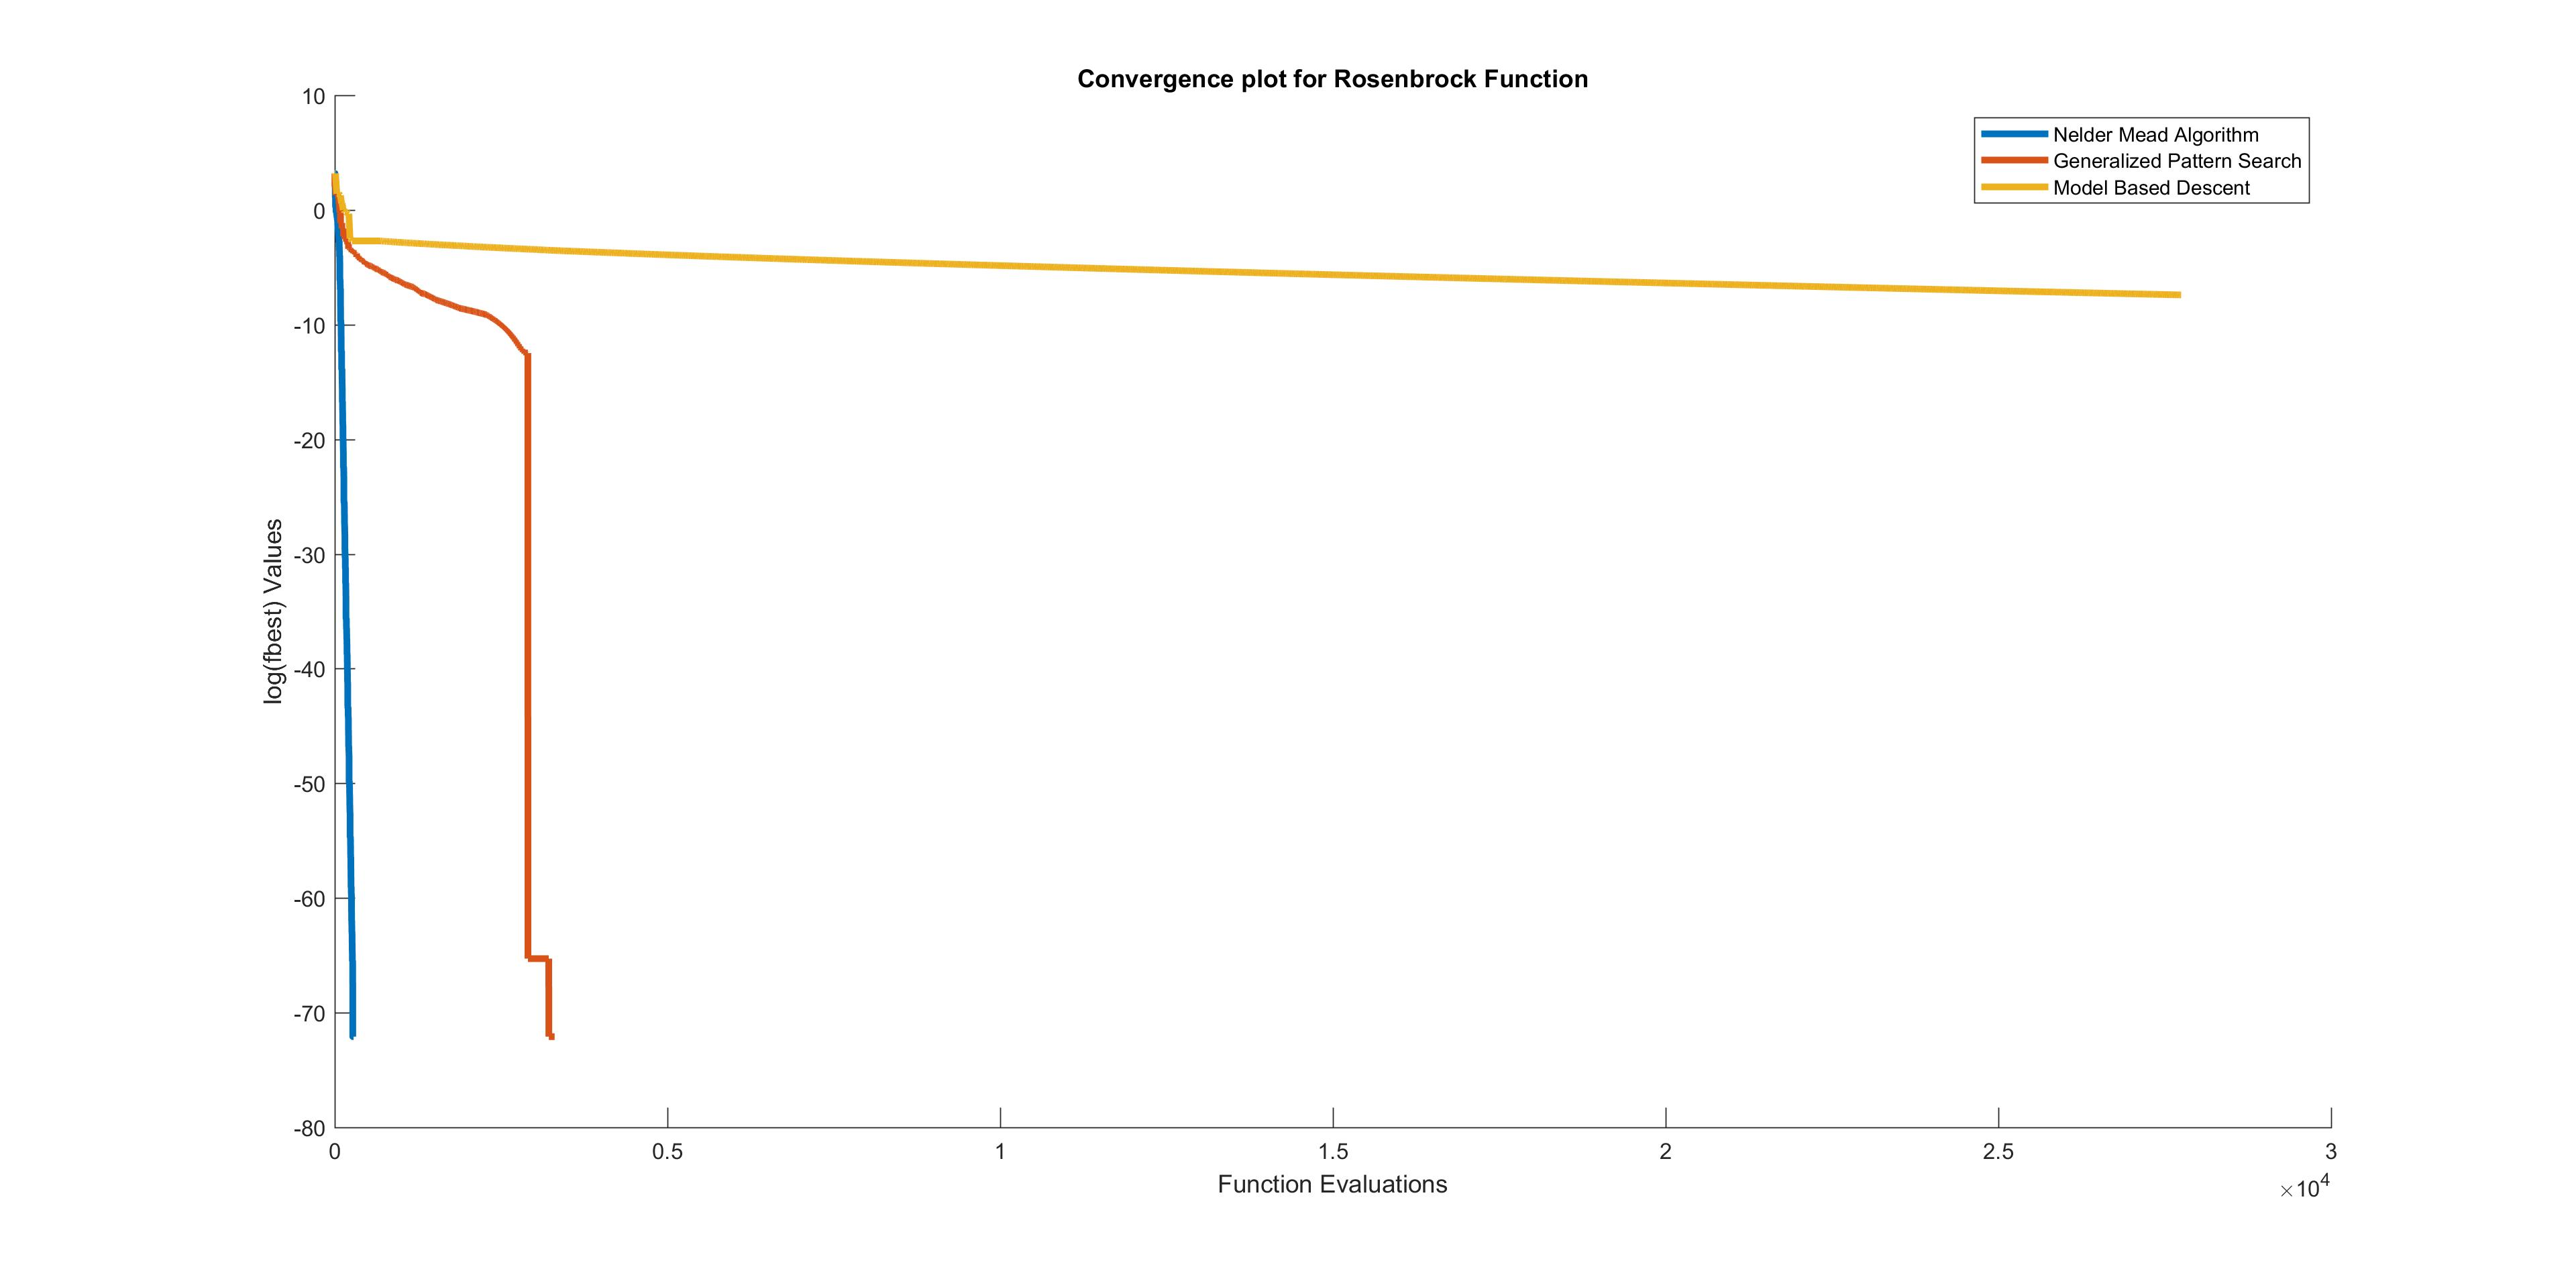
\includegraphics[width=\linewidth]{RosenbrockConvF.jpg}
			\caption{Convergence plot of NM, GPS \& MBD}
		\end{figure}
	\end{frame}
	
	\begin{frame}{Convergence plot}{Cube Function}
		\begin{figure}
			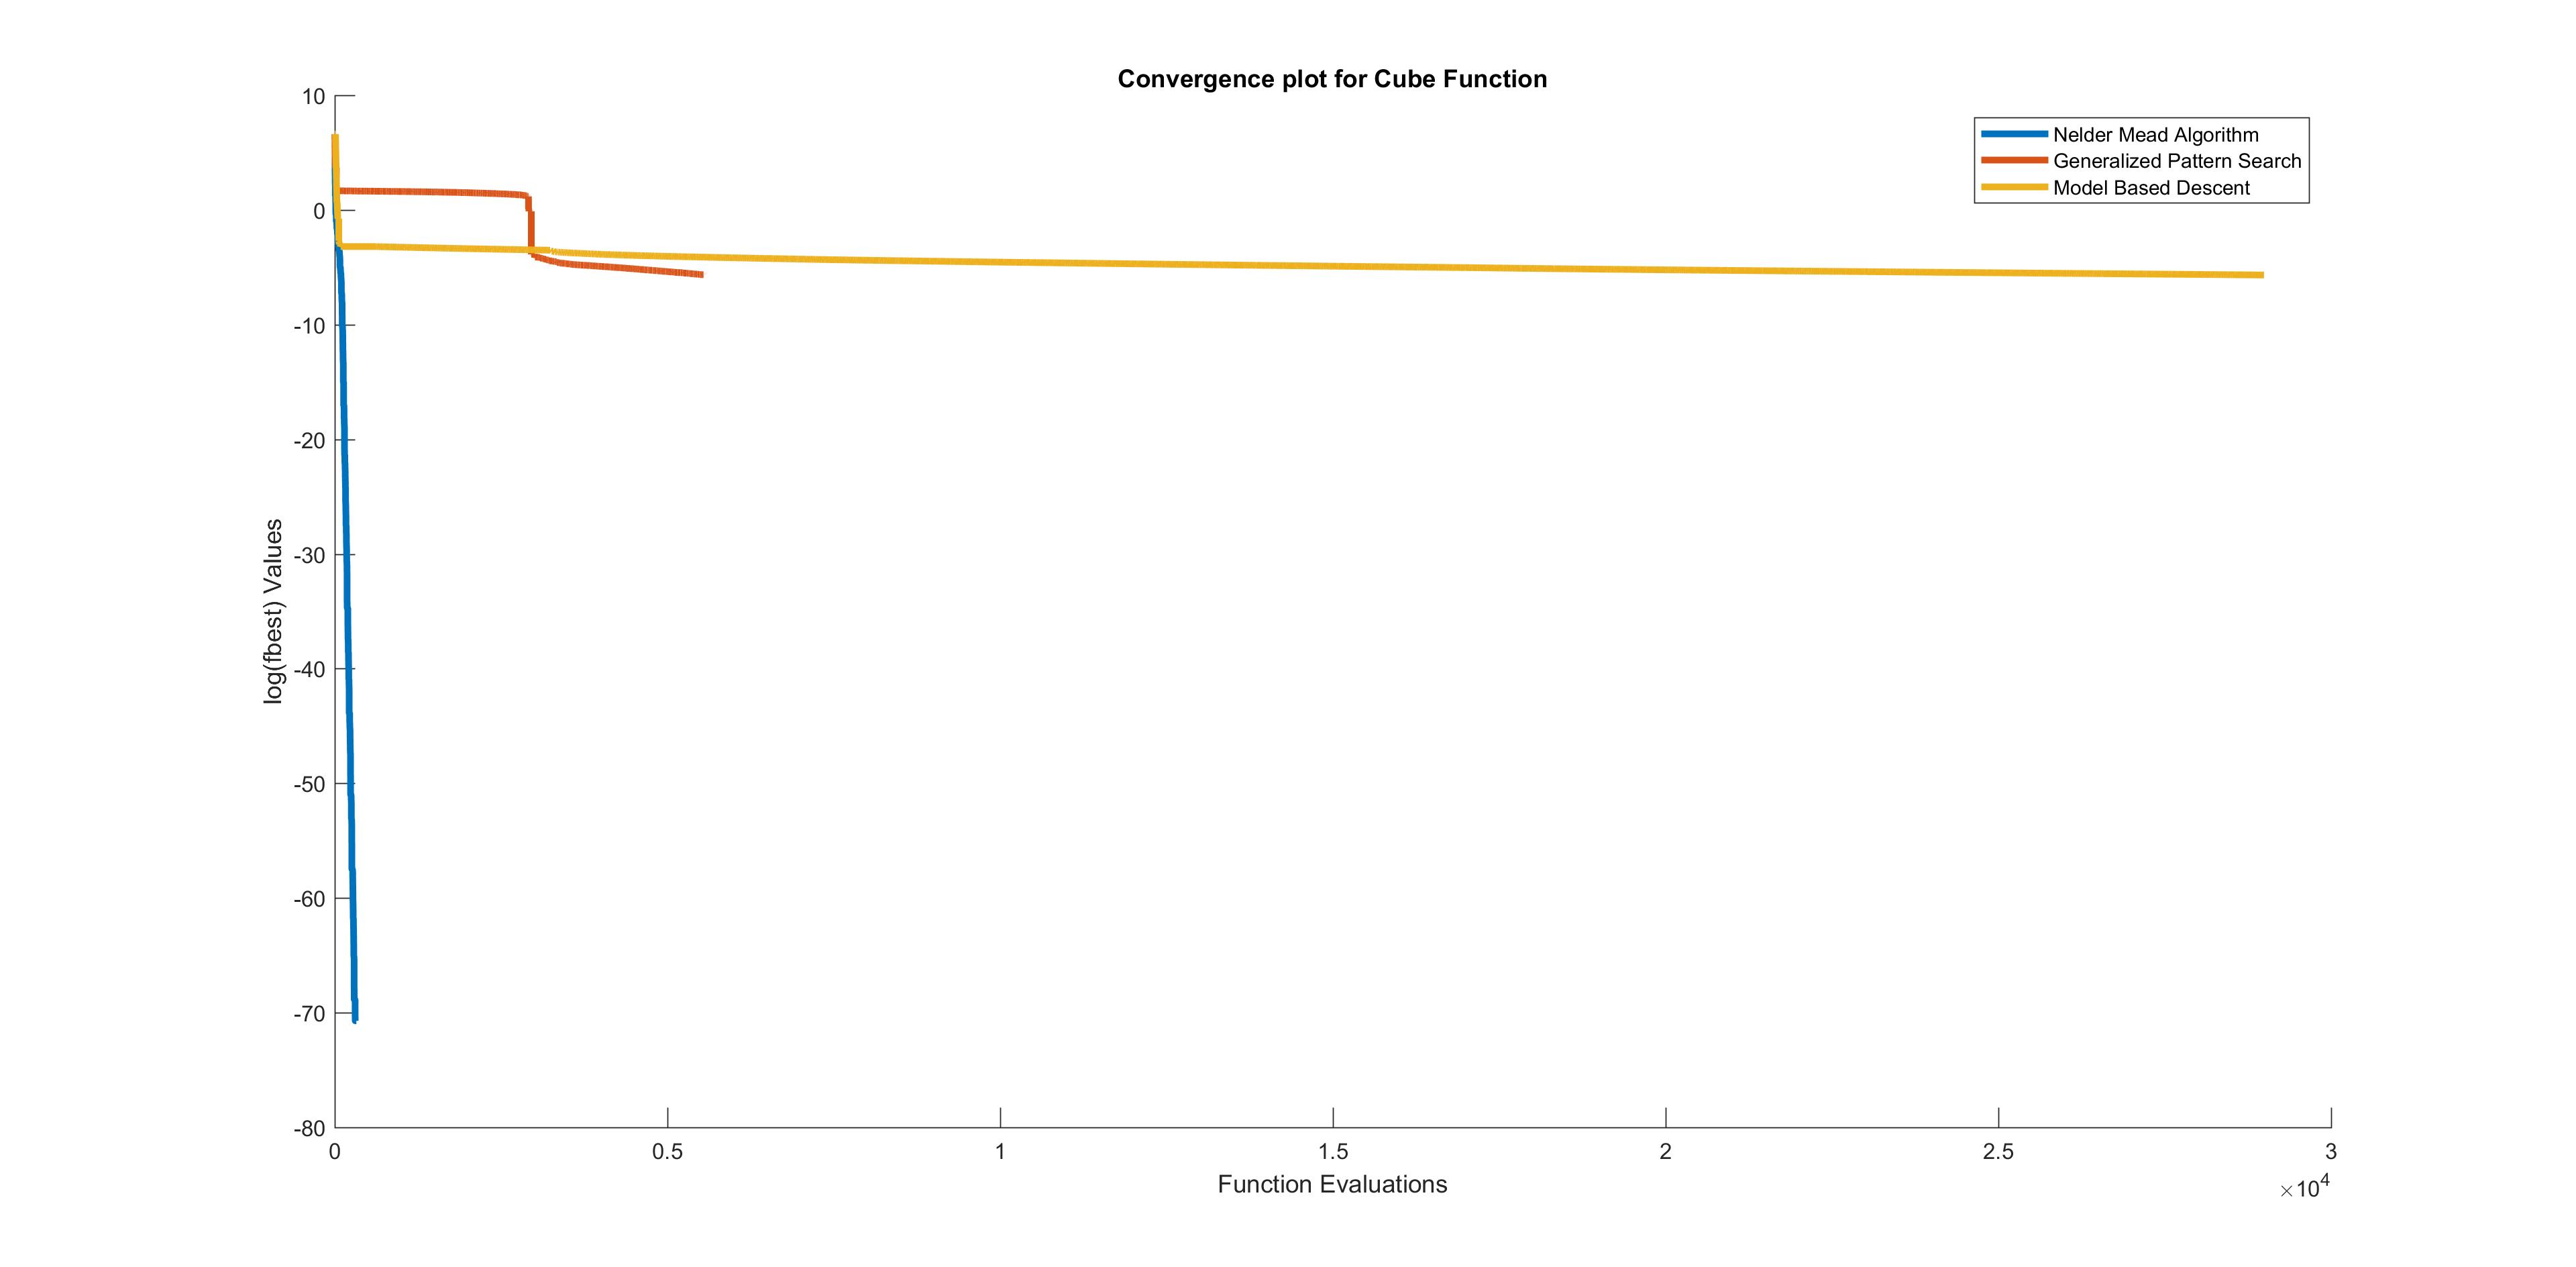
\includegraphics[width=\linewidth]{CubeConvF.jpg}
			\caption{Convergence plot of NM, GPS \& MBD}
		\end{figure}
	\end{frame}
	
	\begin{frame}{Convergence plot}{Modified Box Function}
		\begin{figure}
			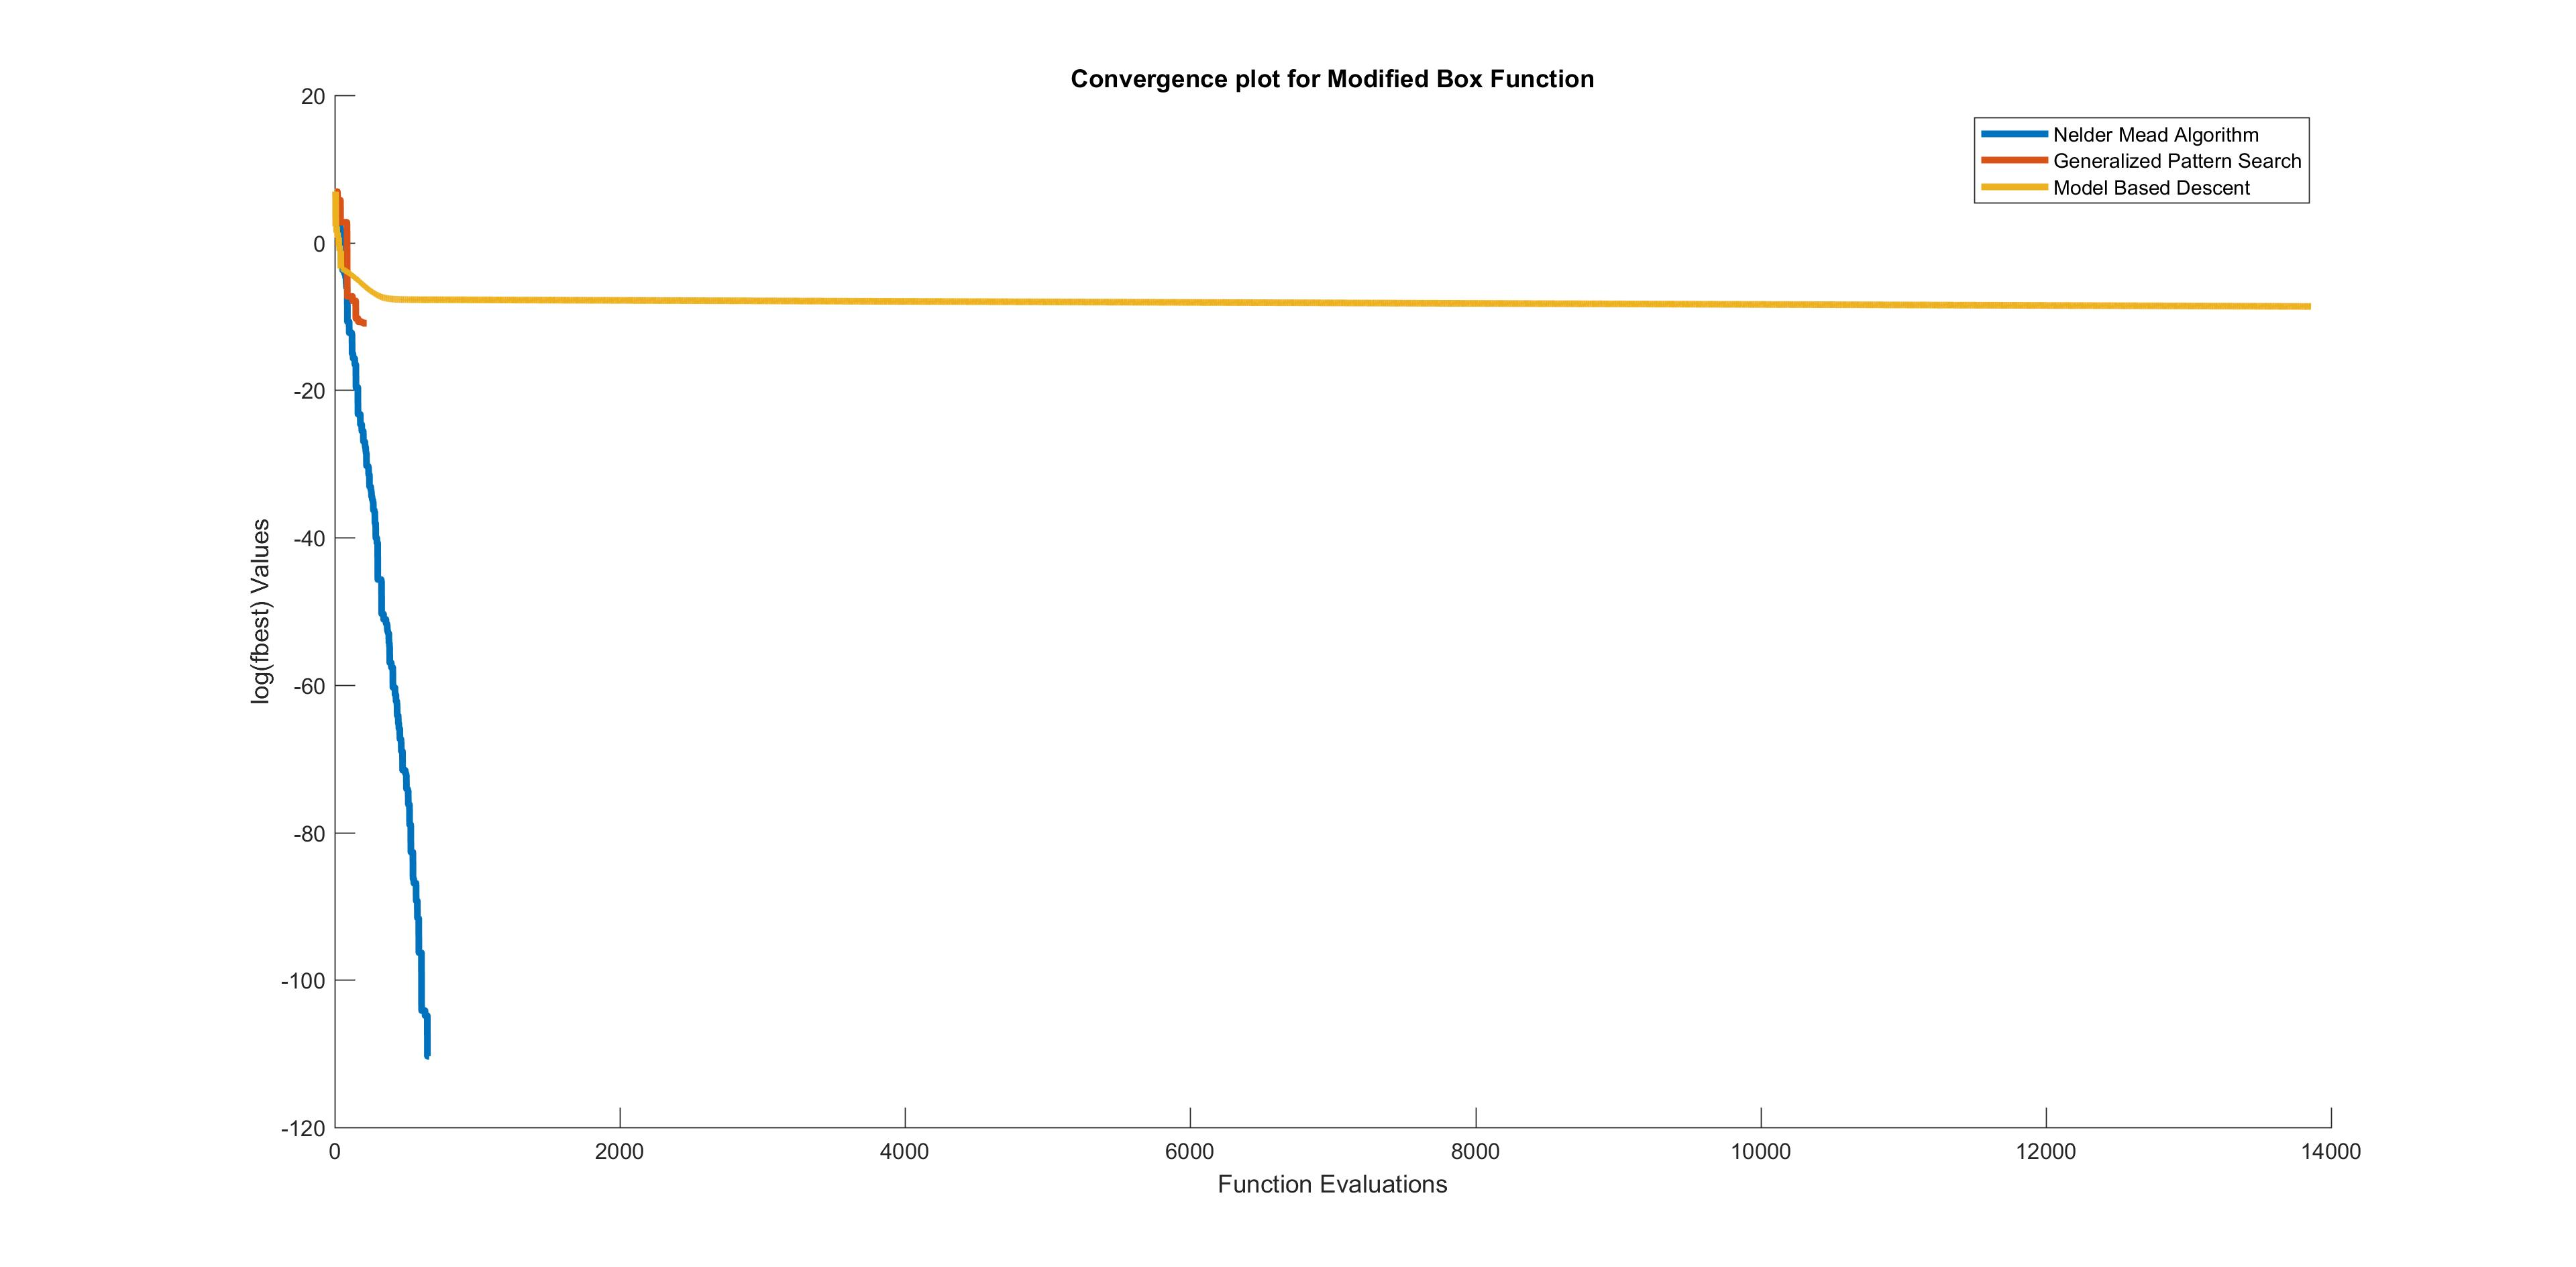
\includegraphics[width=\linewidth]{mBoxConvF.jpg}
			\caption{Convergence plot of NM, GPS \& MBD}
		\end{figure}
	\end{frame}

	\begin{frame}{Convergence plot}{Enzyme/Kowalik Osborne I Function}
		\begin{figure}
			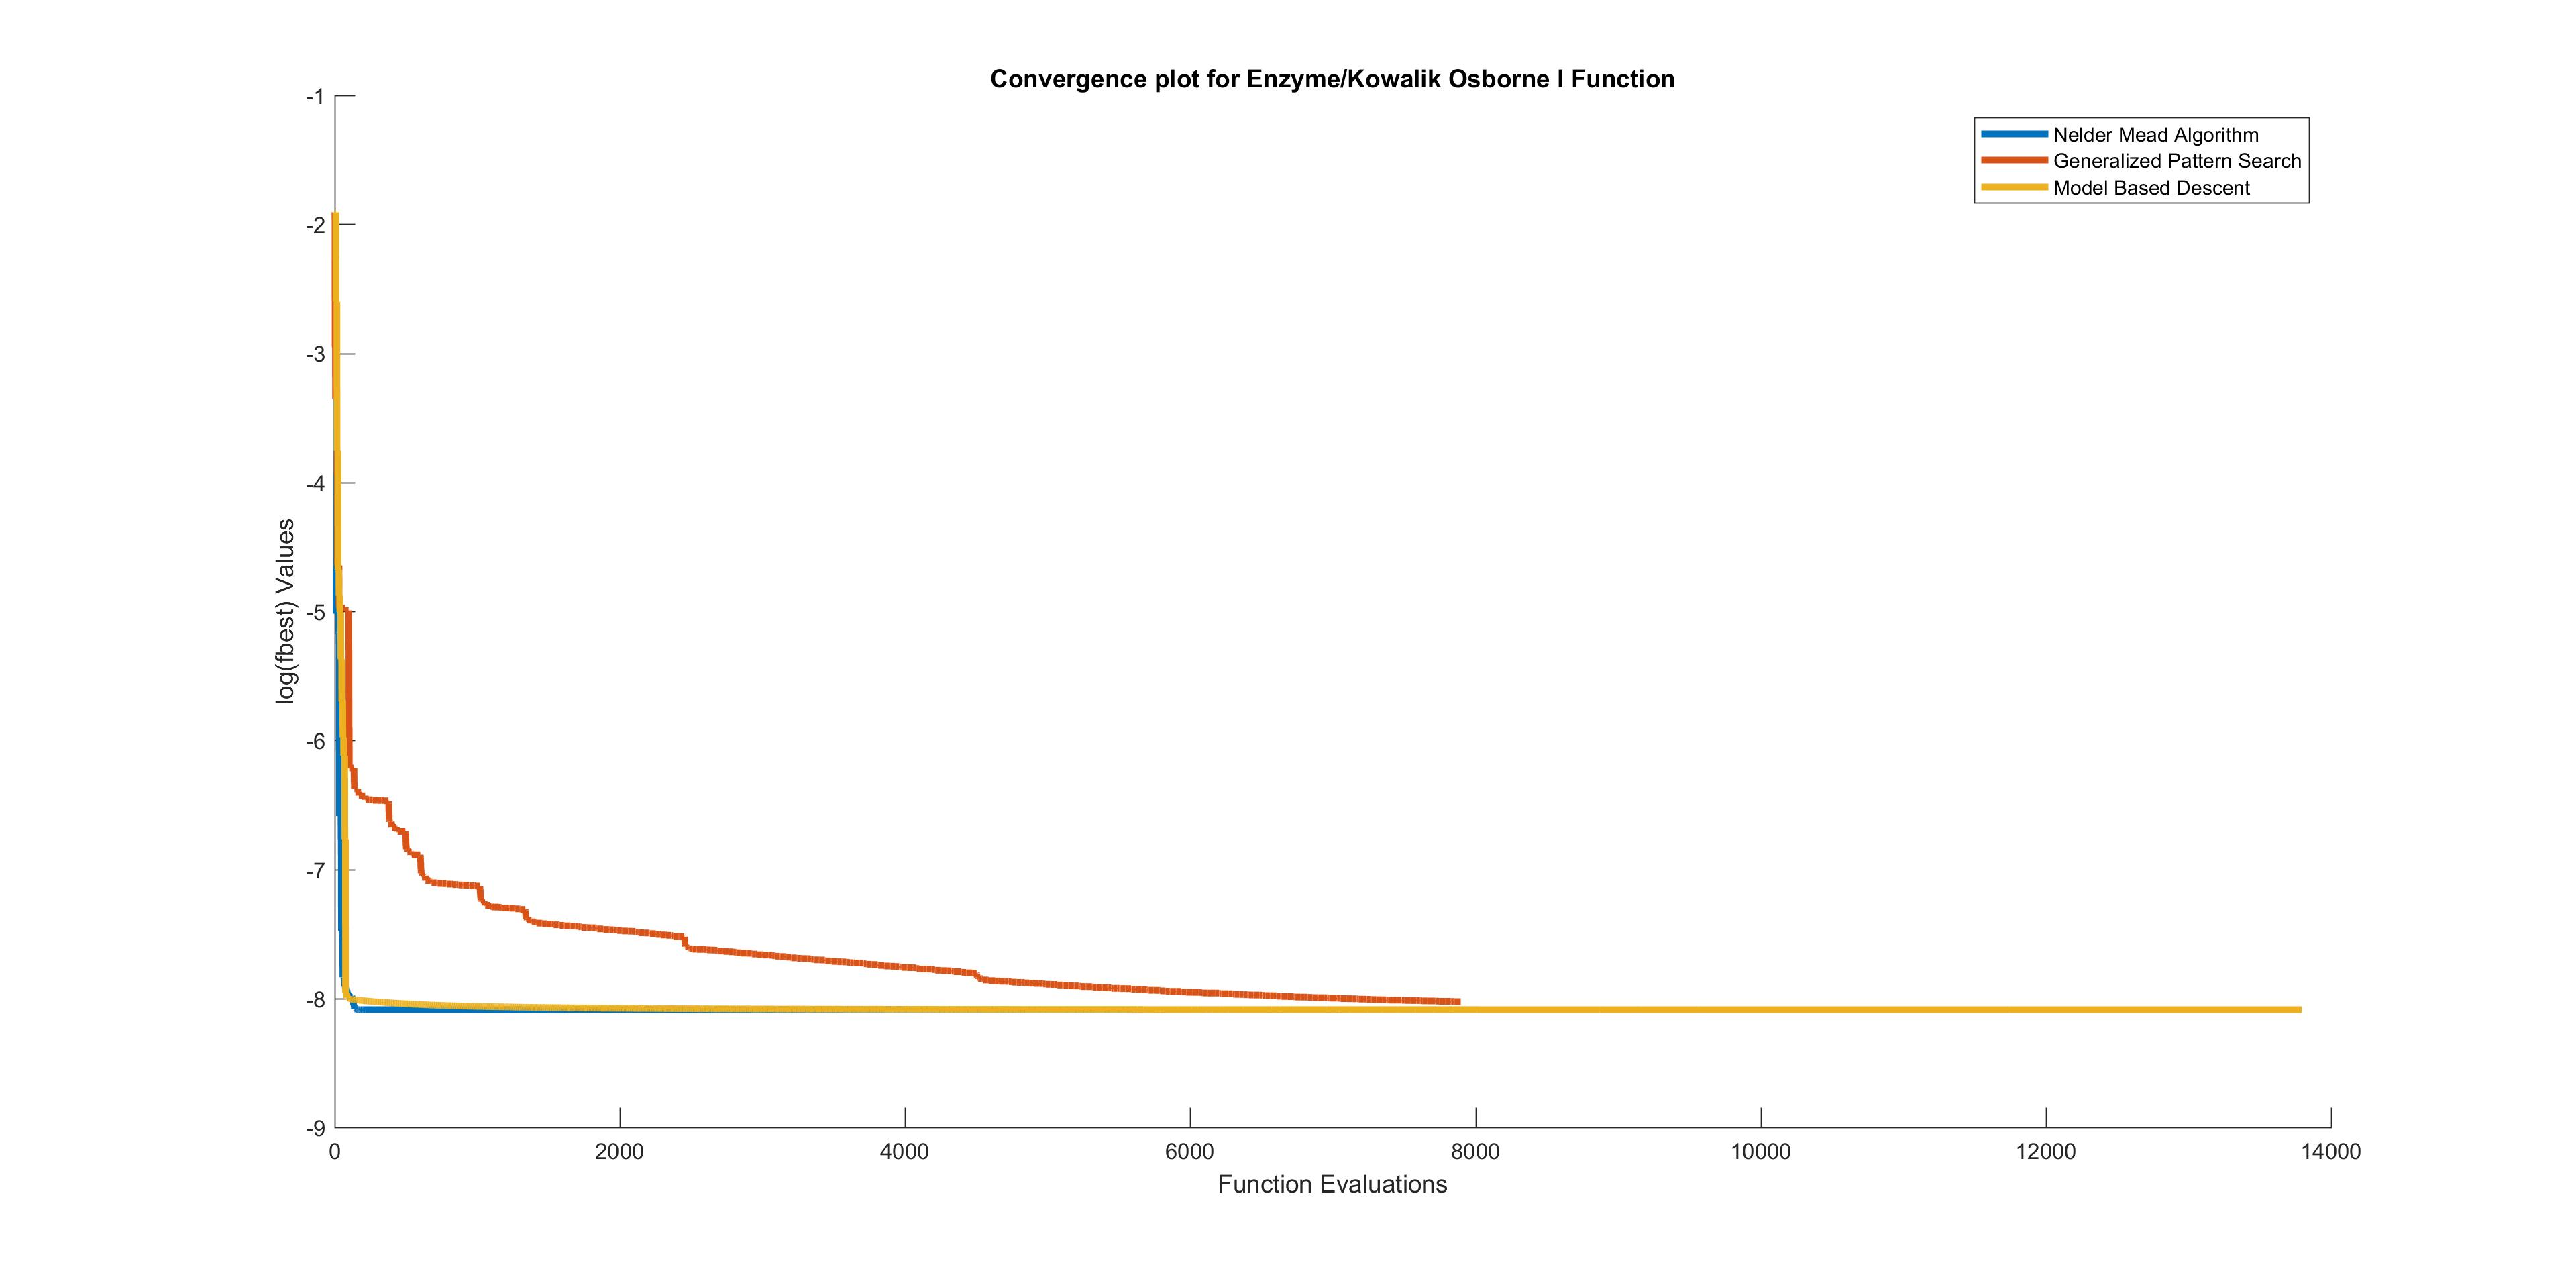
\includegraphics[width=\linewidth]{koConvF.jpg}
			\caption{Convergence plot of NM, GPS \& MBD}
		\end{figure}
	\end{frame}
	
	\begin{frame}{Trajectory Plot}{Rosenbrock Function}
		\begin{figure}
			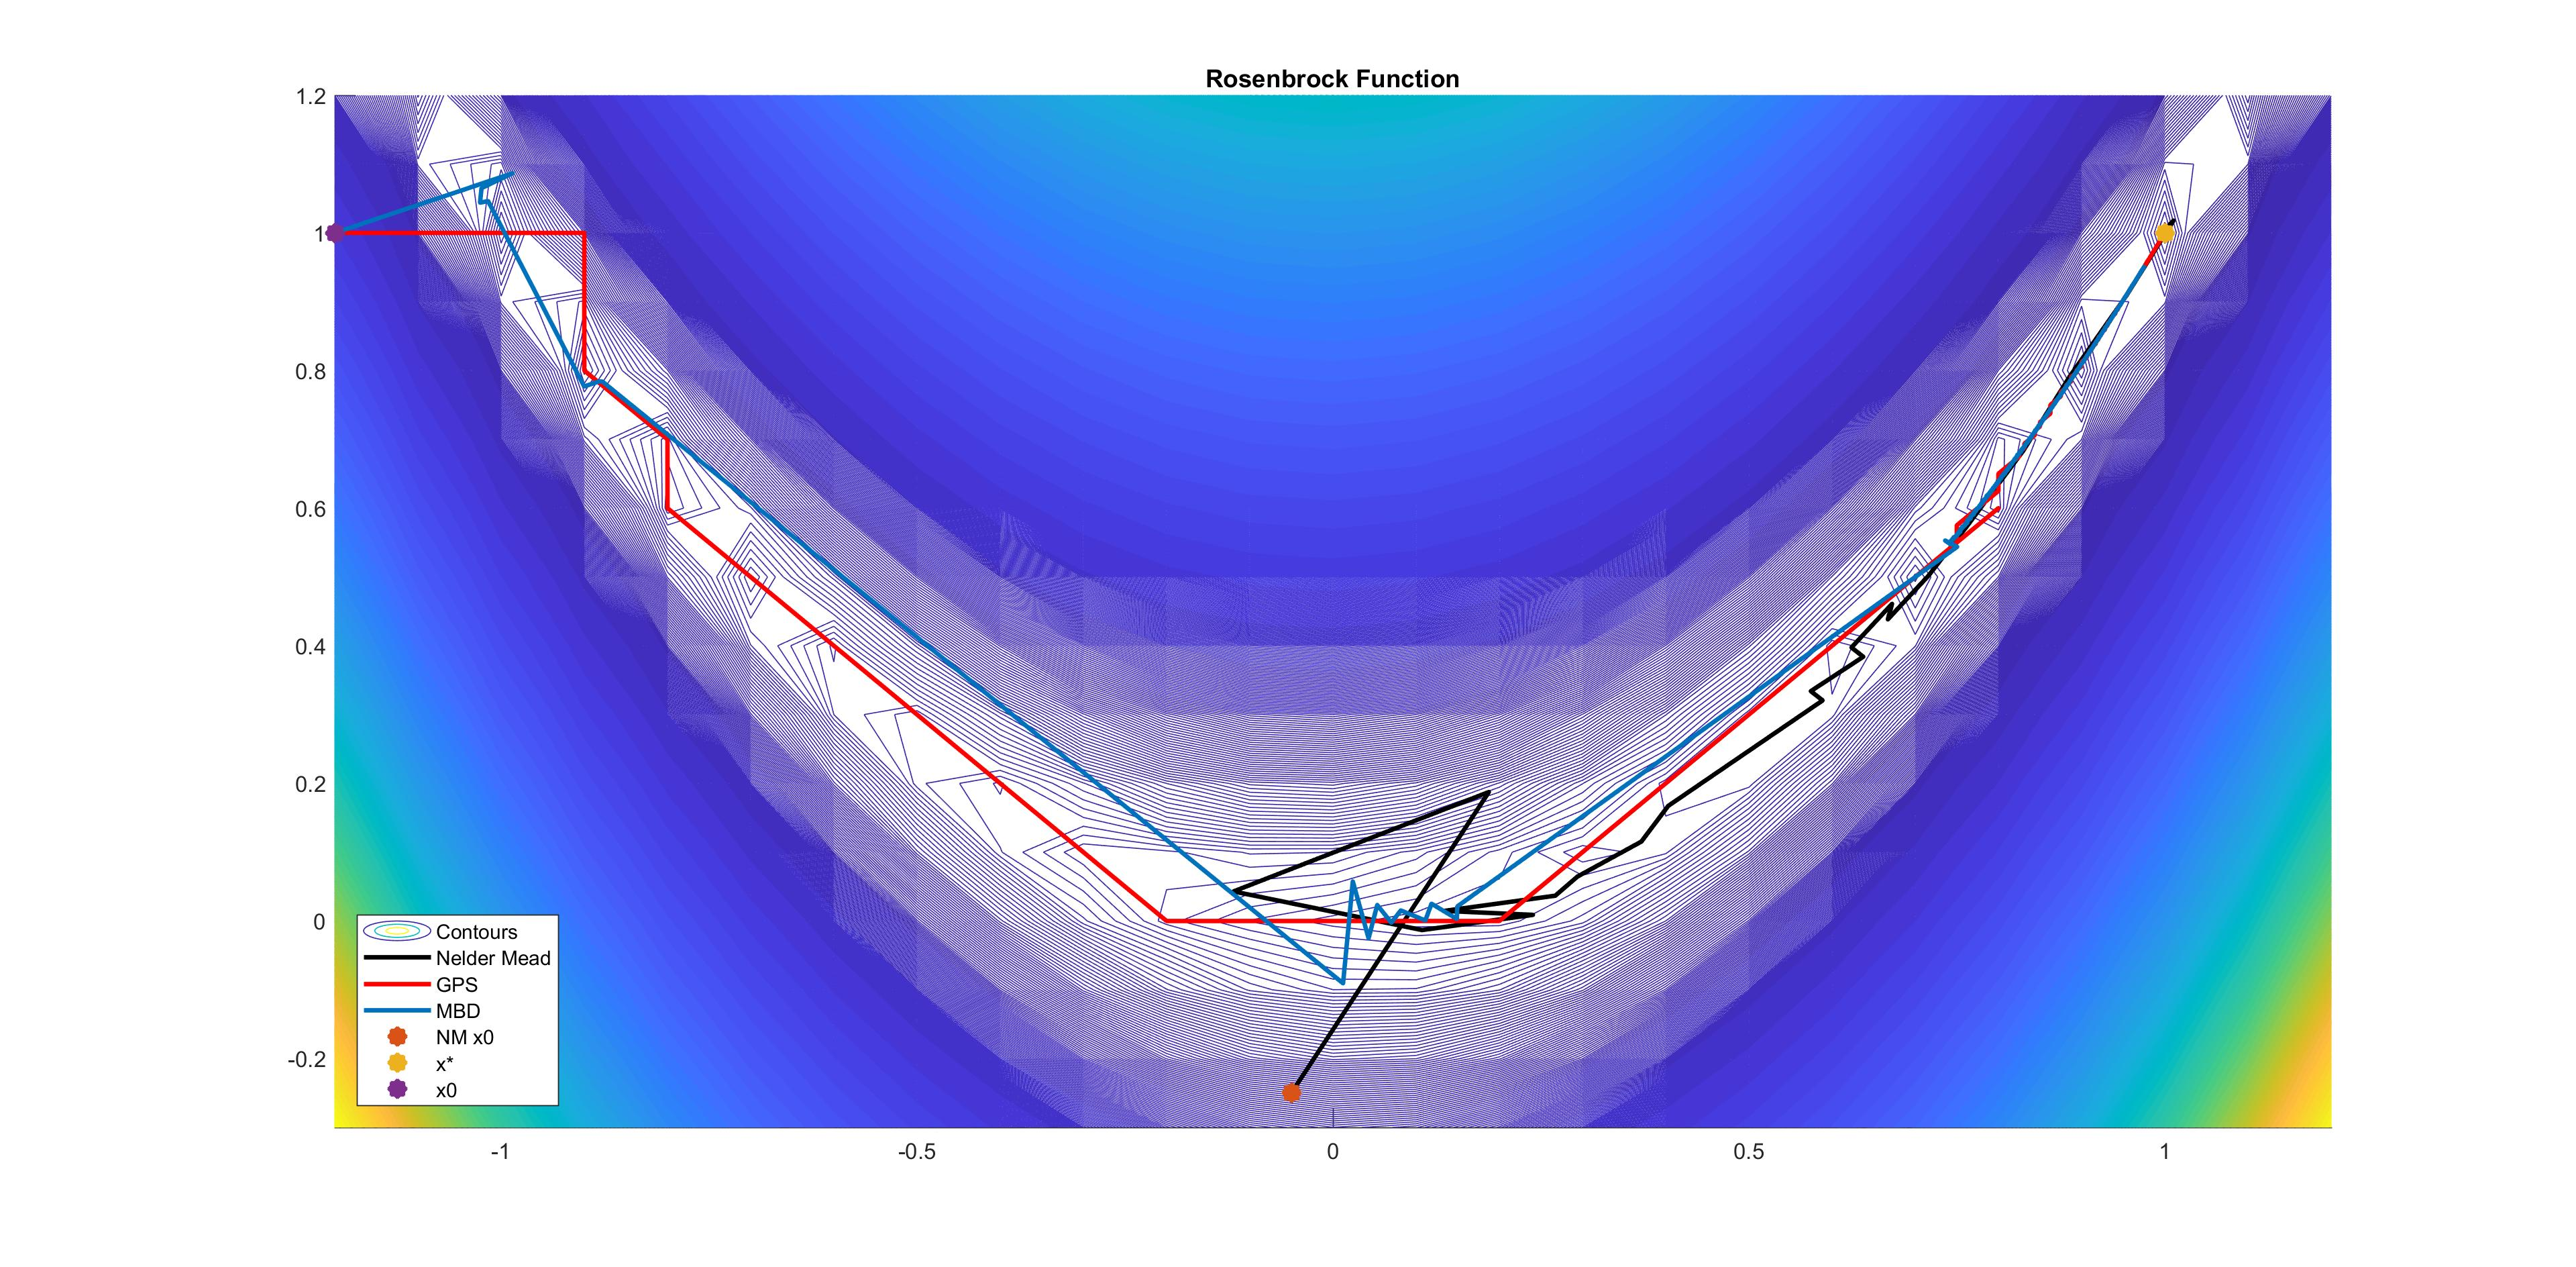
\includegraphics[width=\linewidth]{RosenbrockContour.jpg}
			\caption{Algorithmic Paths of NM, GPS \& MBD}
		\end{figure}
	\end{frame}
	
	\begin{frame}{Trajectory Plot}{Cube Function}
		\begin{figure}
			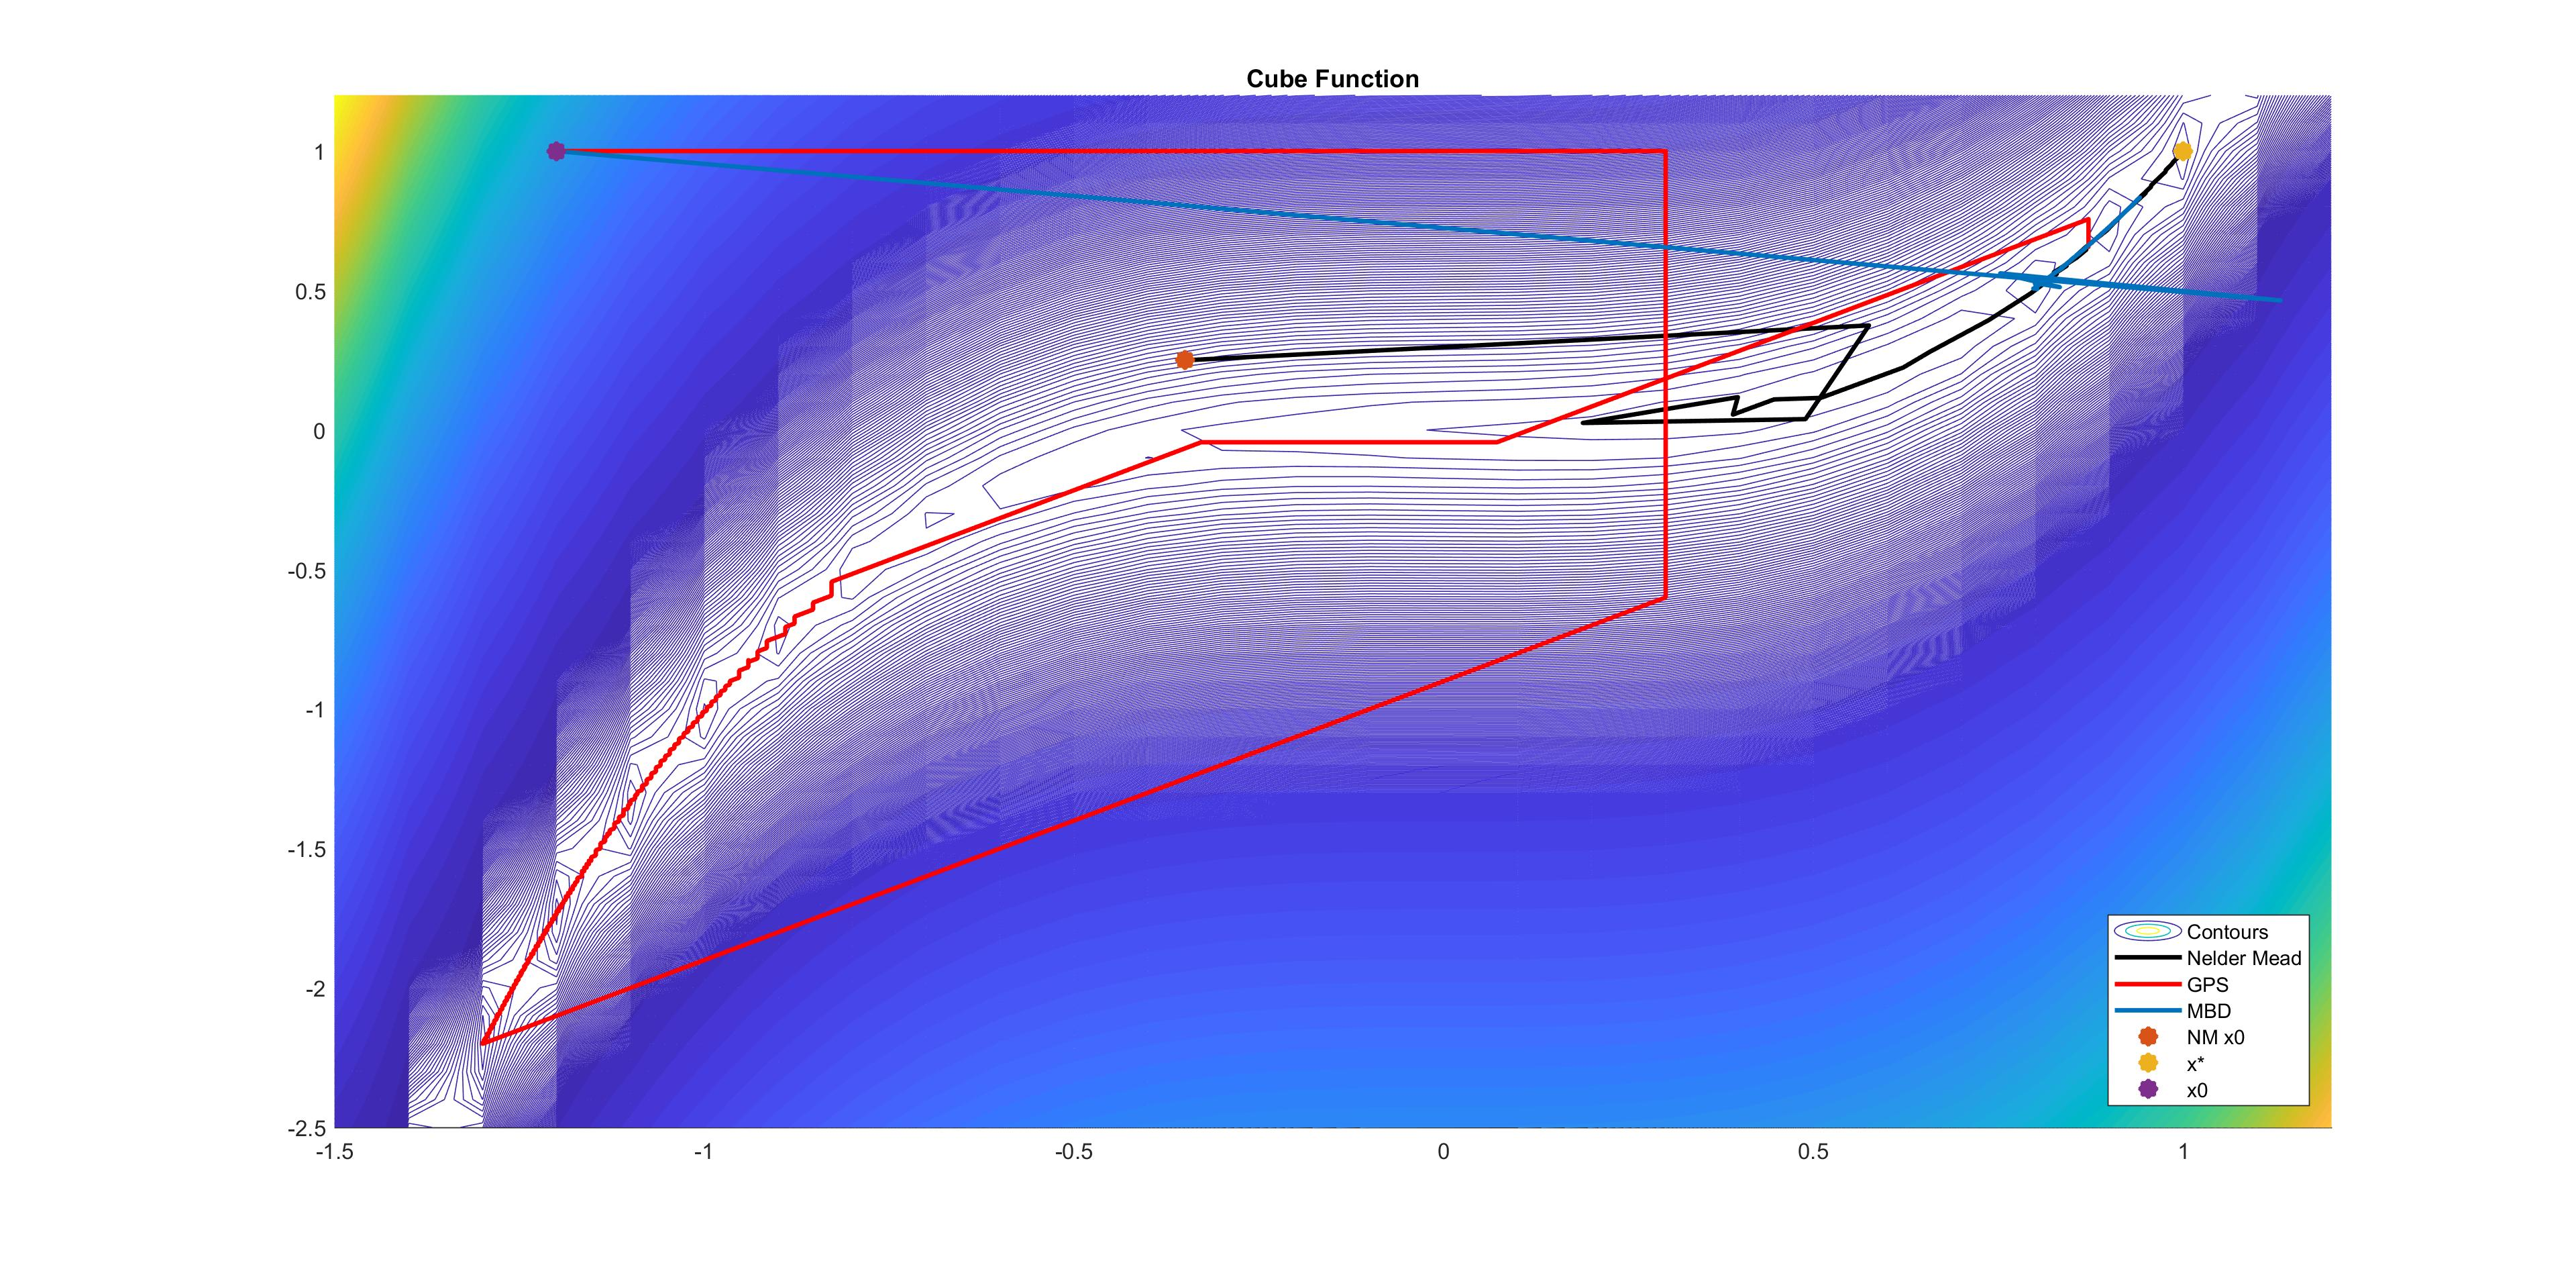
\includegraphics[width=\linewidth]{CubeContour.jpg}
			\caption{Algorithmic Paths of NM, GPS \& MBD}
		\end{figure}
	\end{frame}

	\begin{frame}{Trajectory Plot}{Beale Function}
		\begin{figure}
			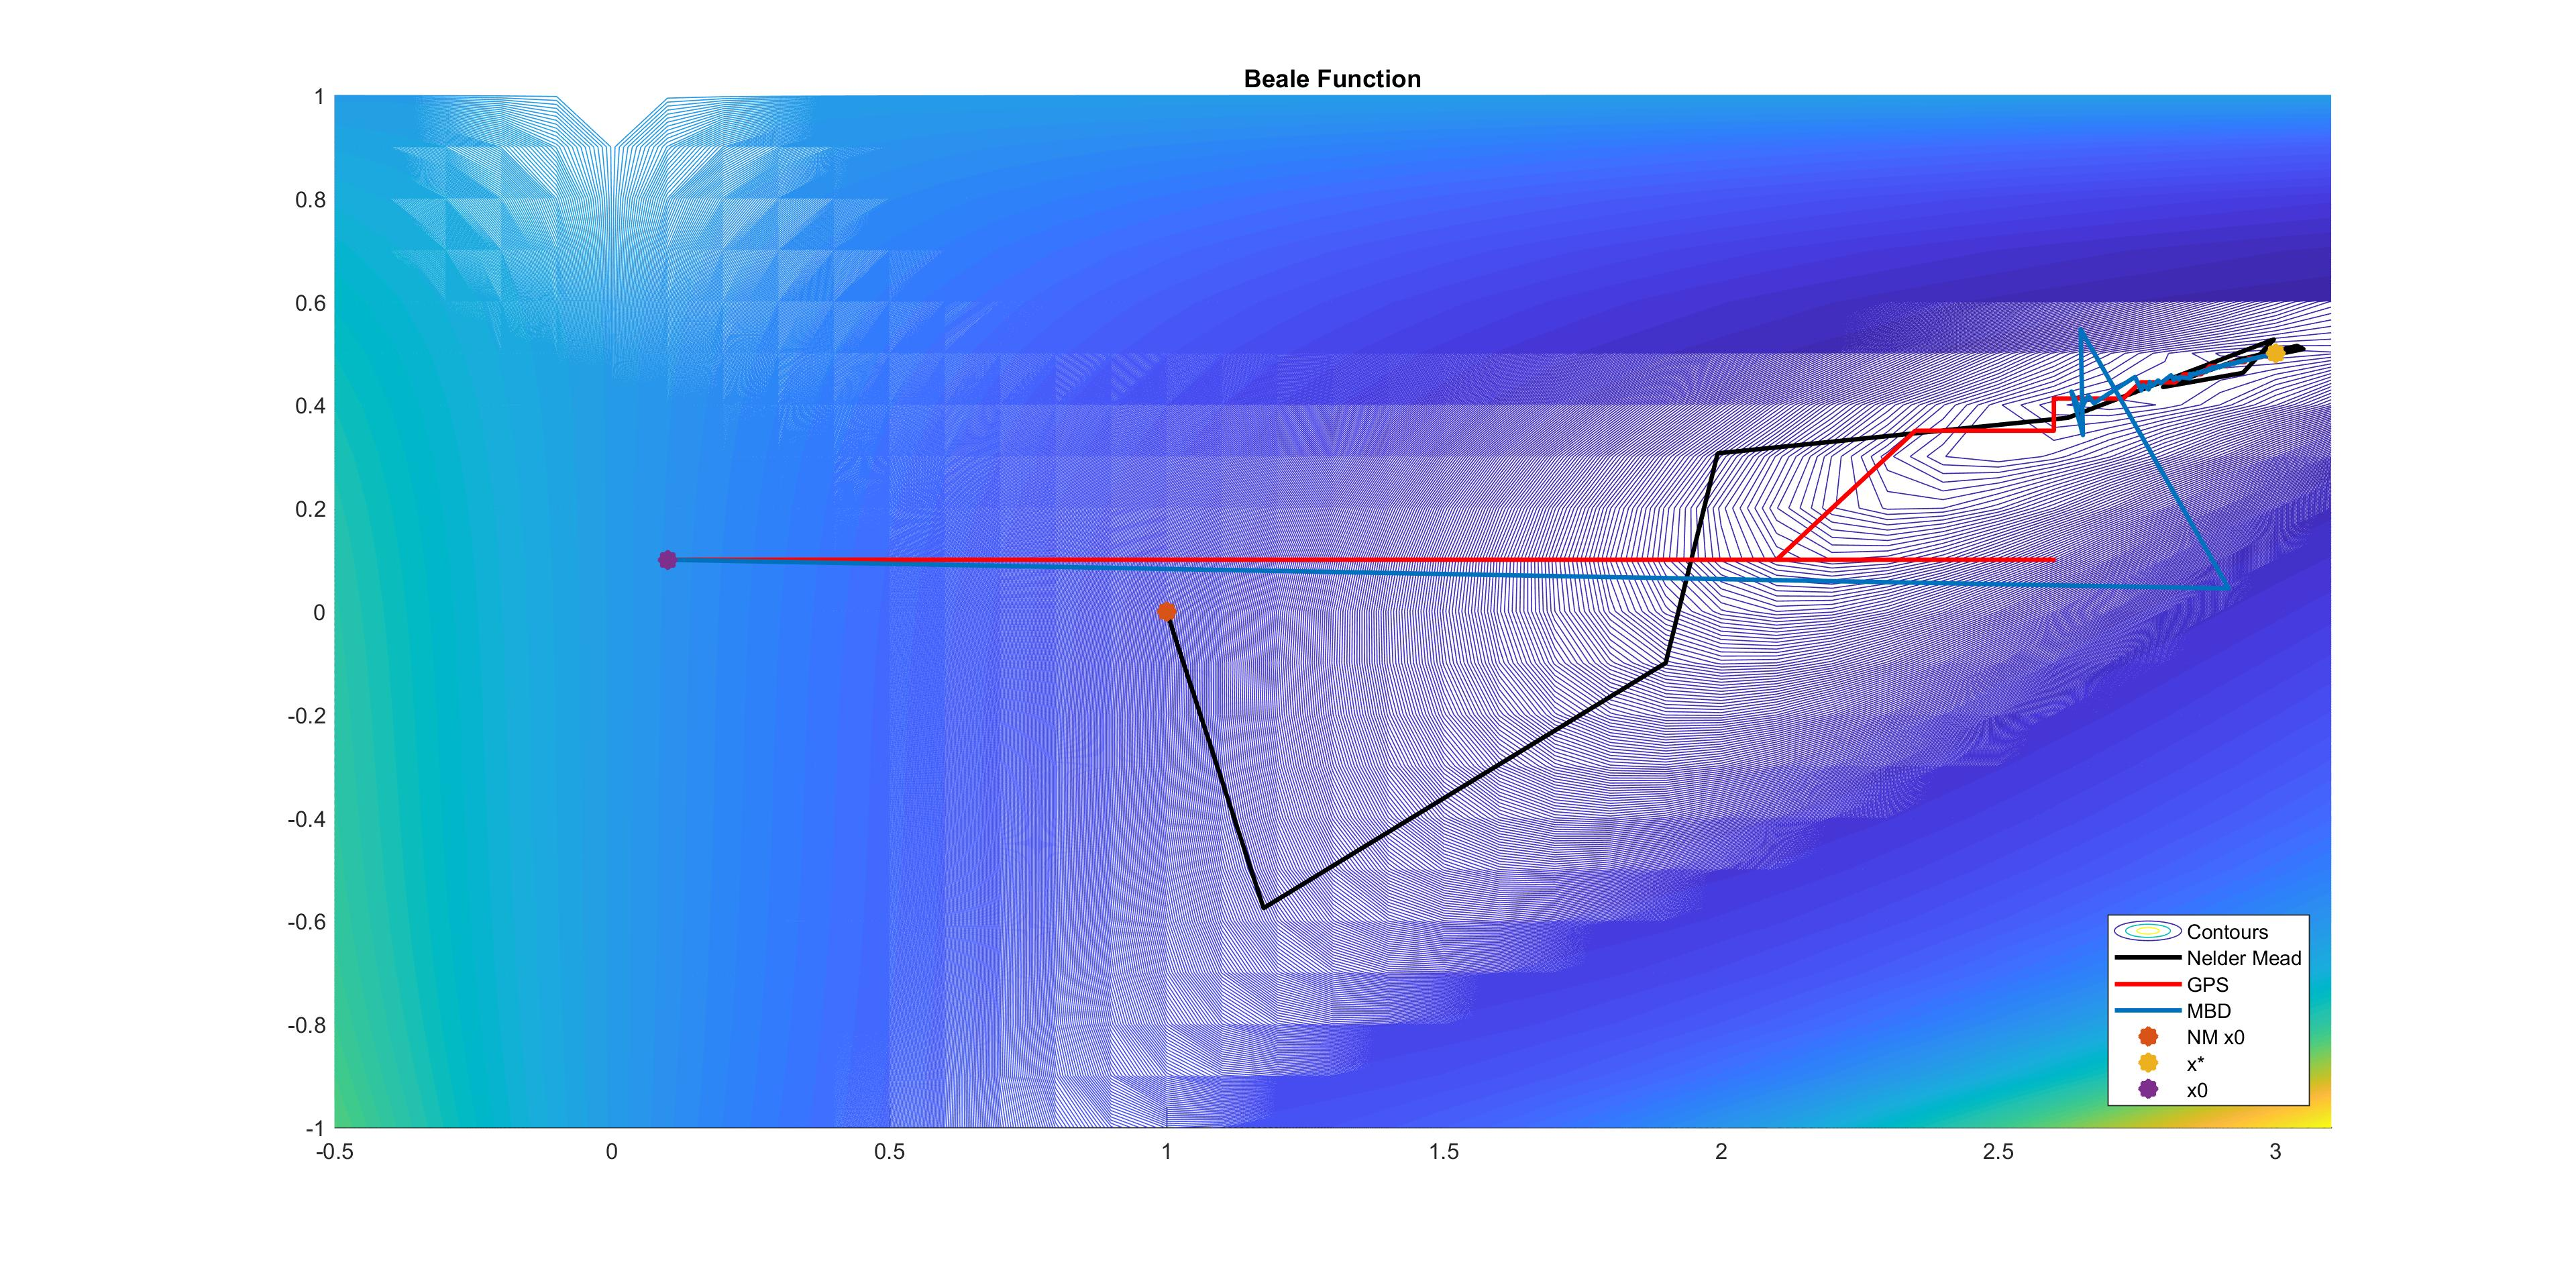
\includegraphics[width=\linewidth]{BealeContour.jpg}
			\caption{Algorithmic Paths of NM, GPS \& MBD}
		\end{figure}
	\end{frame}

	\begin{frame}{Performance Profile}{tau=5\%}
		\begin{figure}
			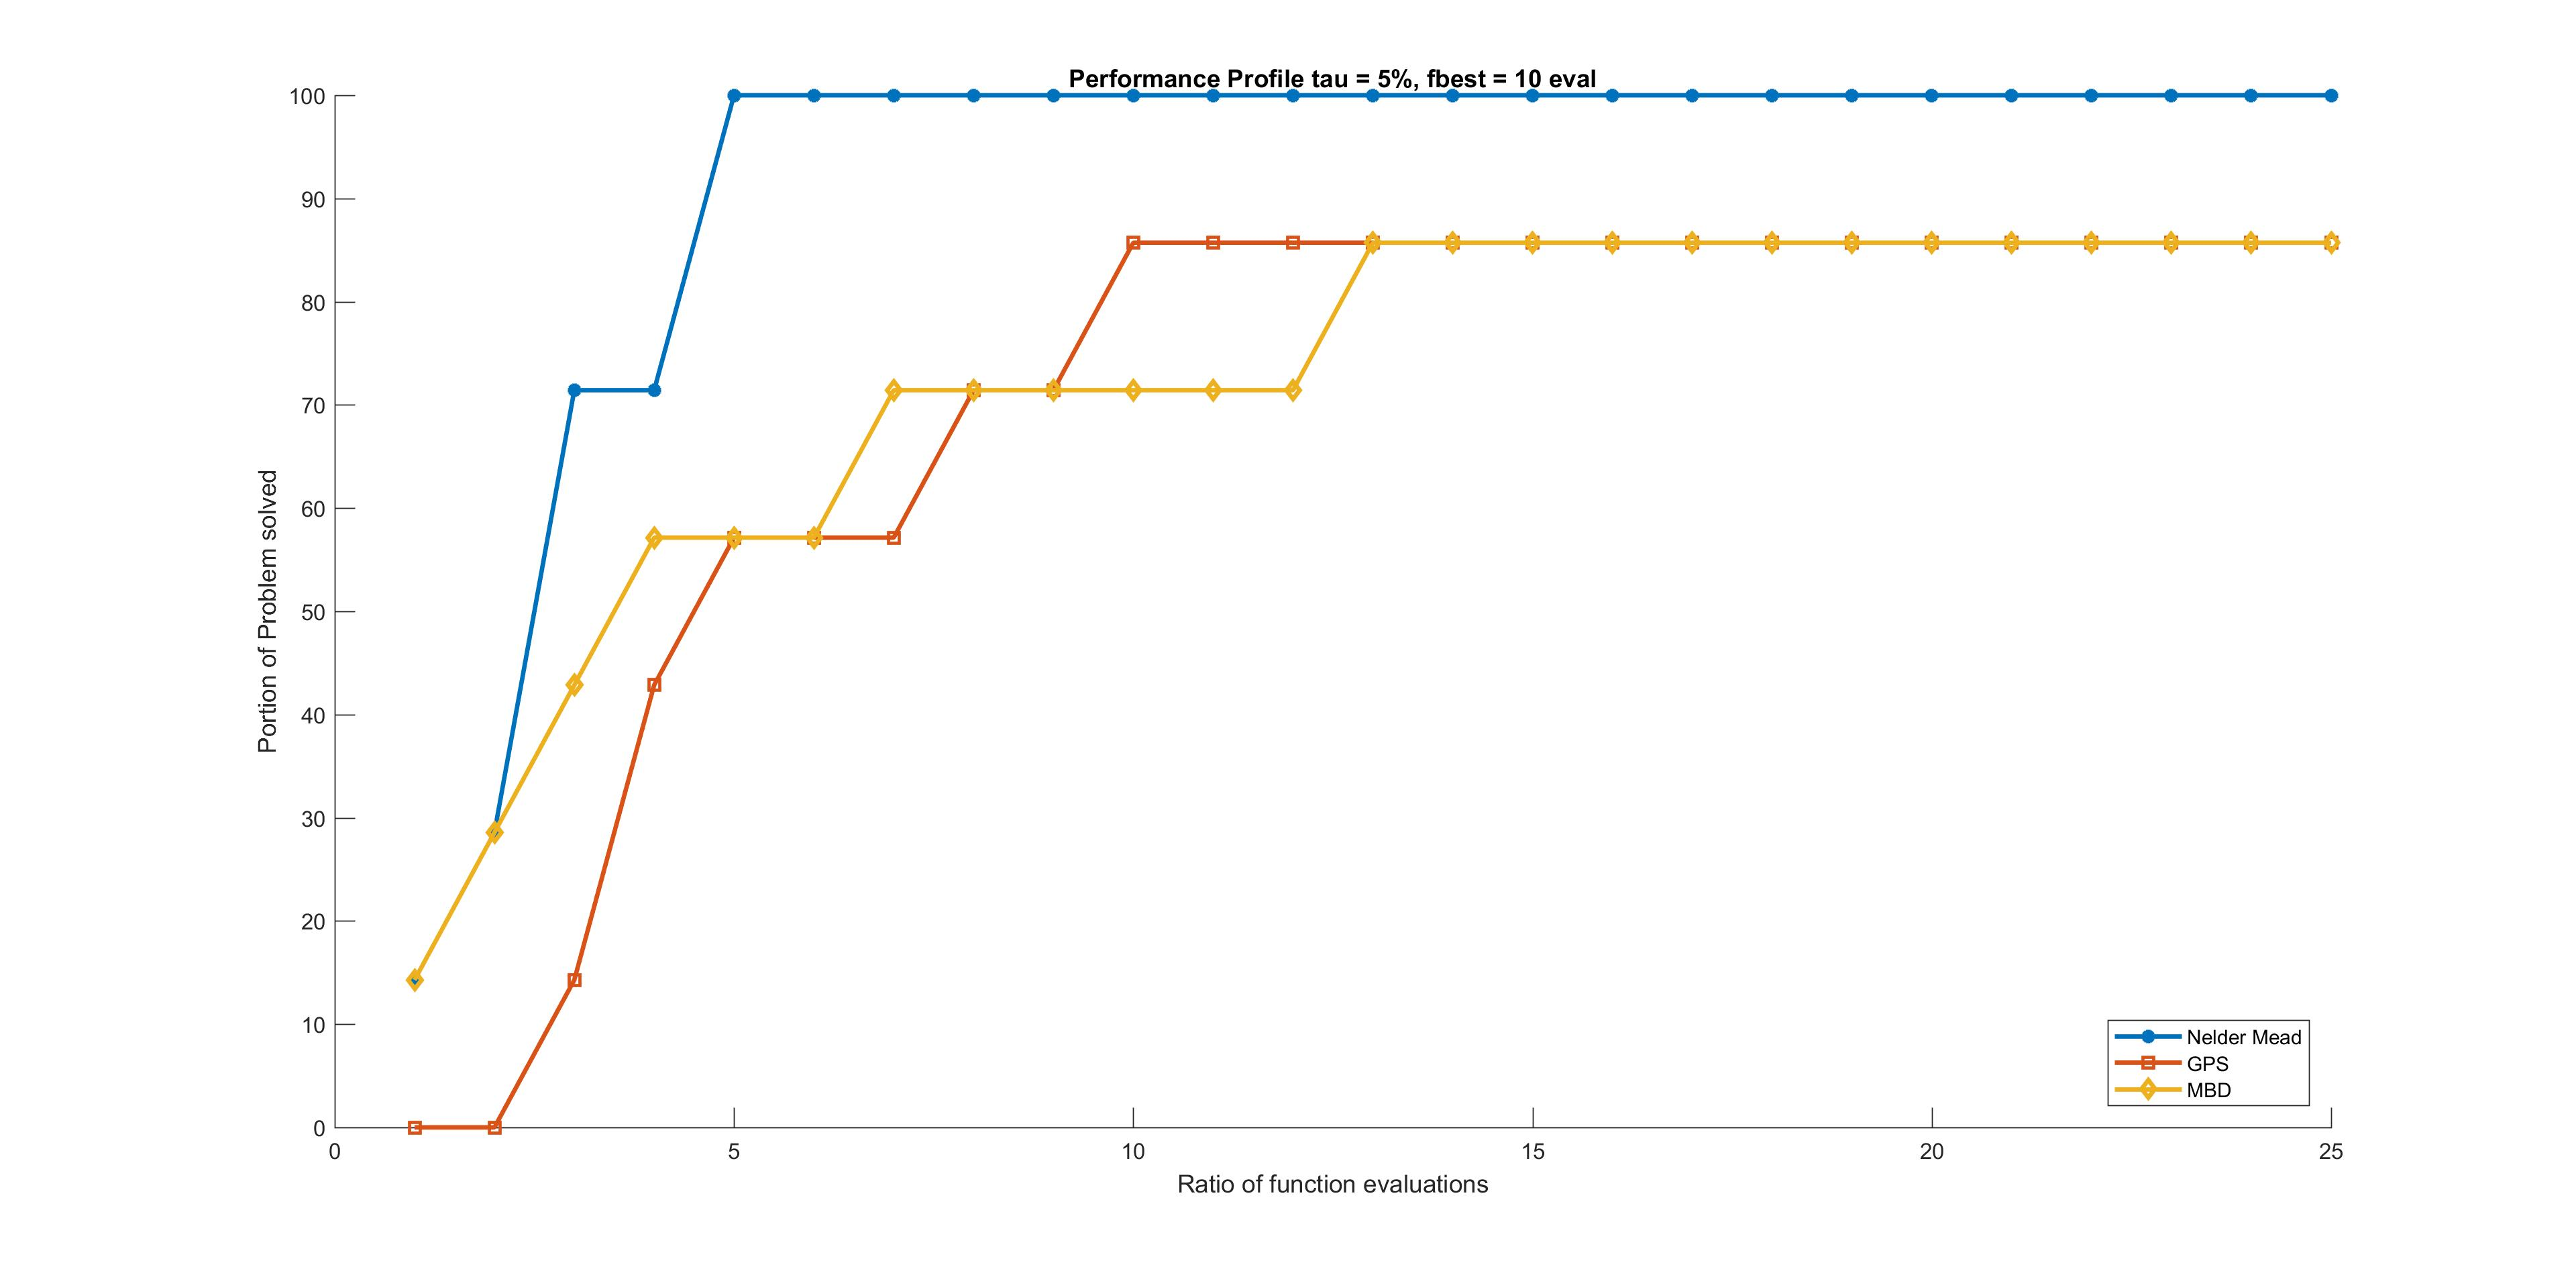
\includegraphics[width=\linewidth]{pptau5.jpg}
			\caption{Performance Profile for NM, GPS \& MBD}
		\end{figure}
	\end{frame}
	
	\begin{frame}{Performance Profile}{tau=10\%}
		\begin{figure}
			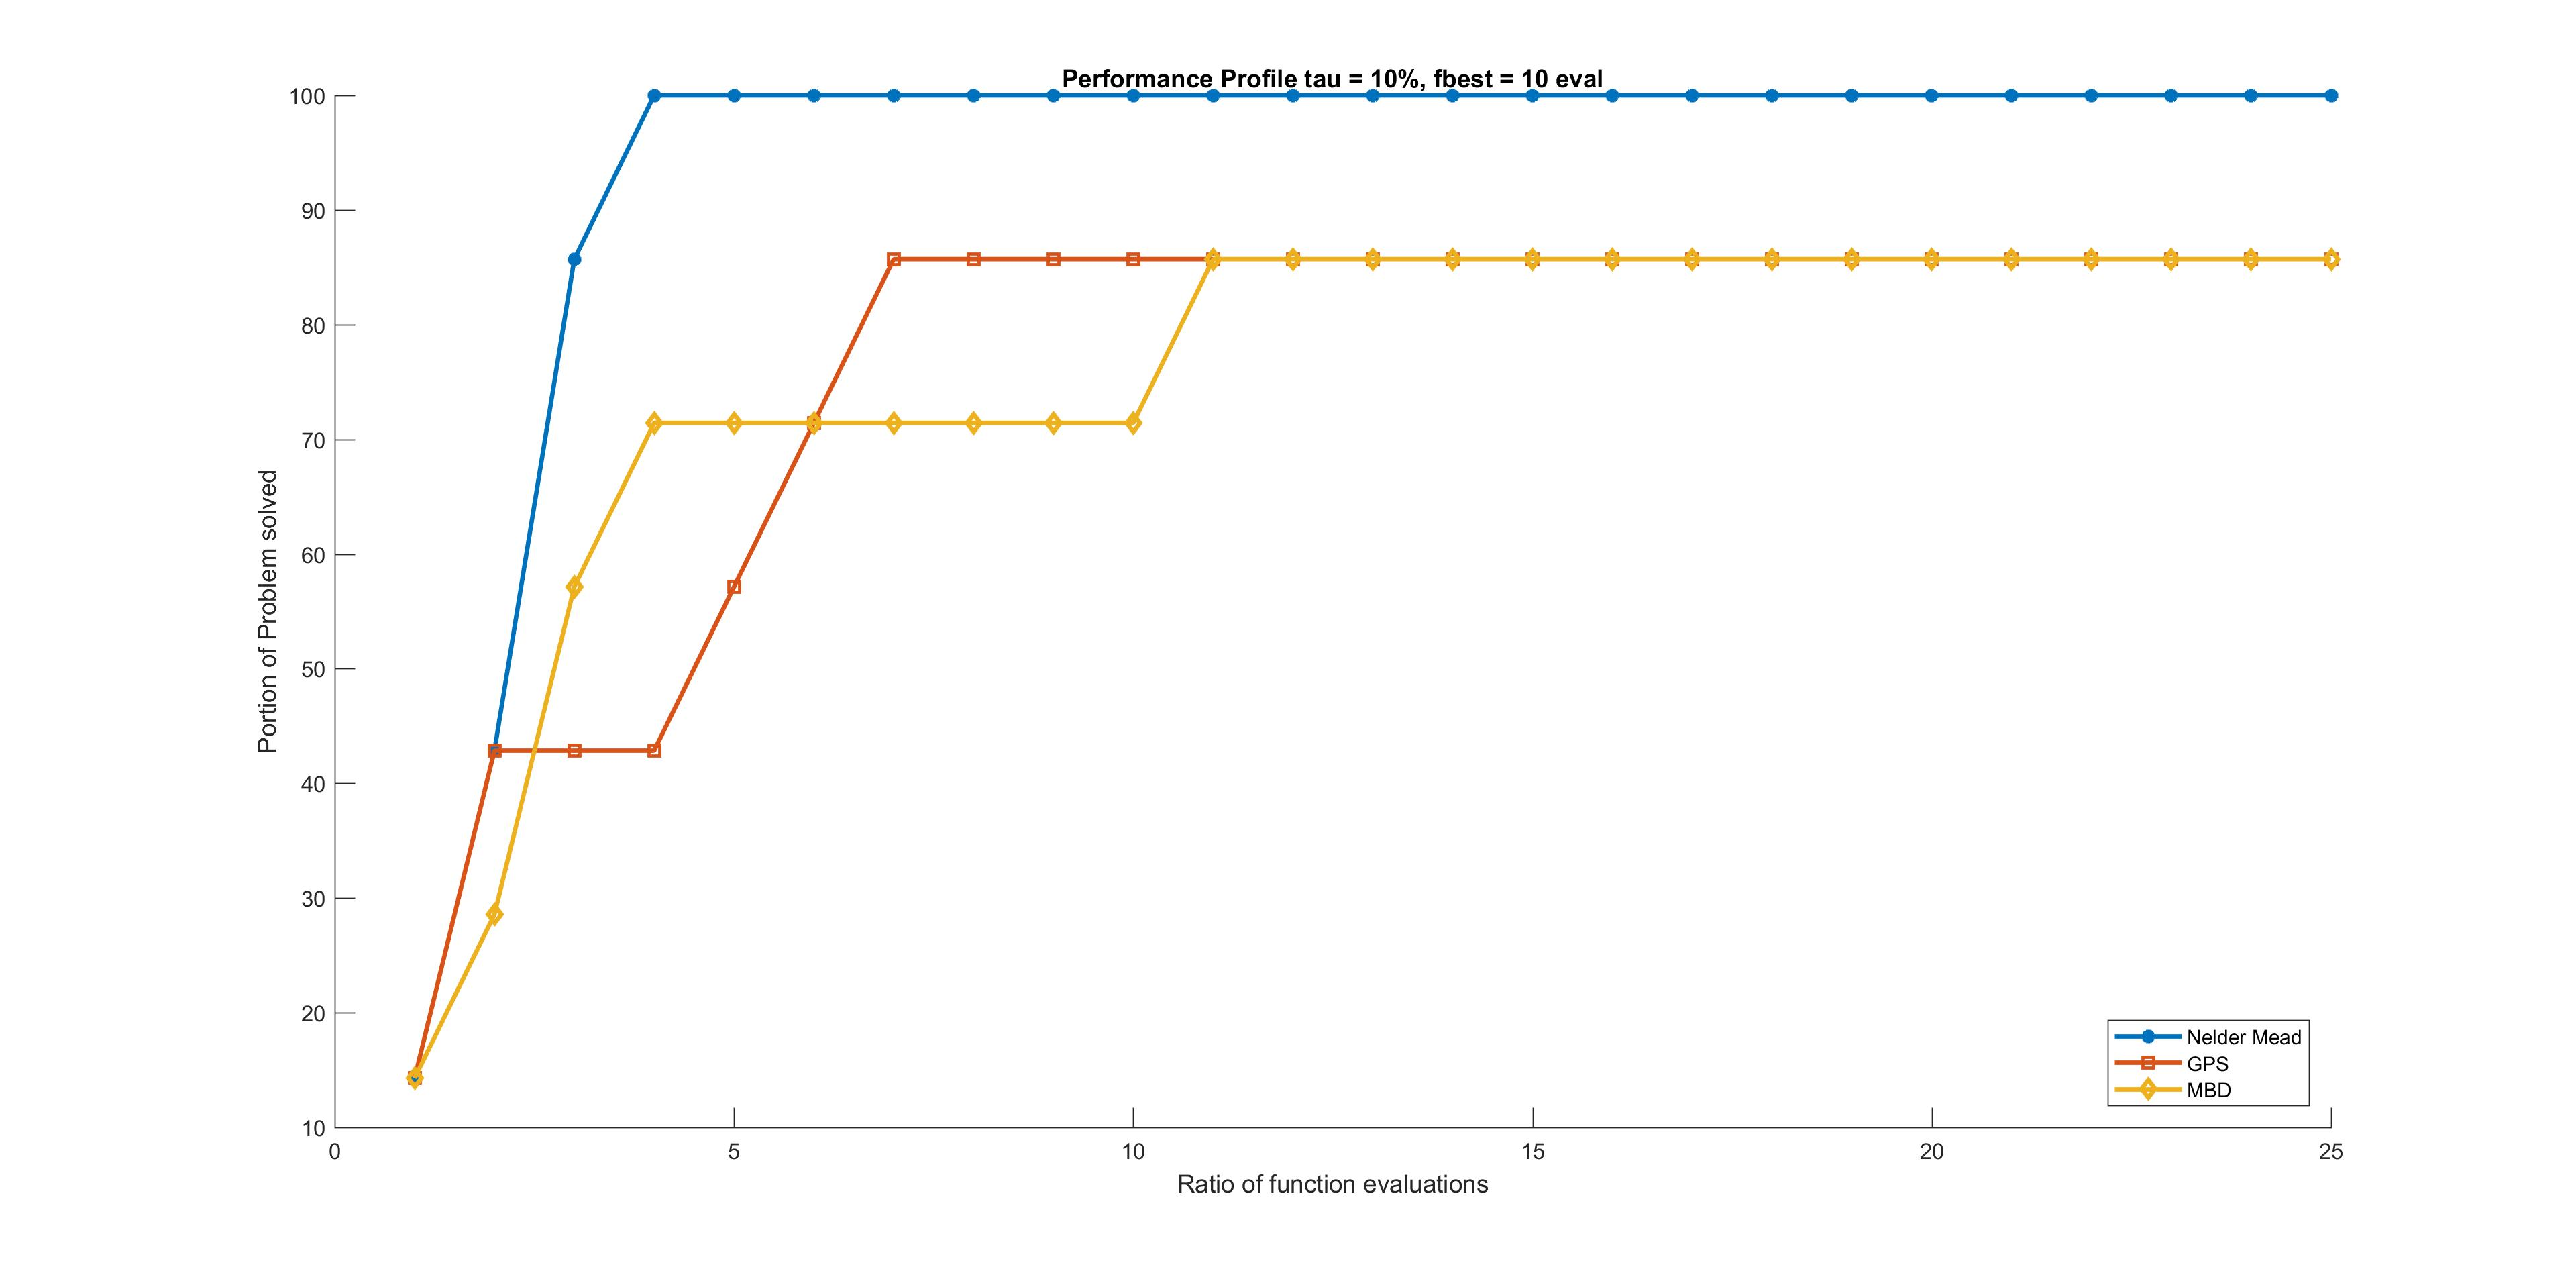
\includegraphics[width=\linewidth]{pptau10.jpg}
			\caption{Performance Profile for NM, GPS \& MBD}
		\end{figure}
	\end{frame}

	\begin{frame}{Data Profile}{tau=5\%}
		\begin{figure}
			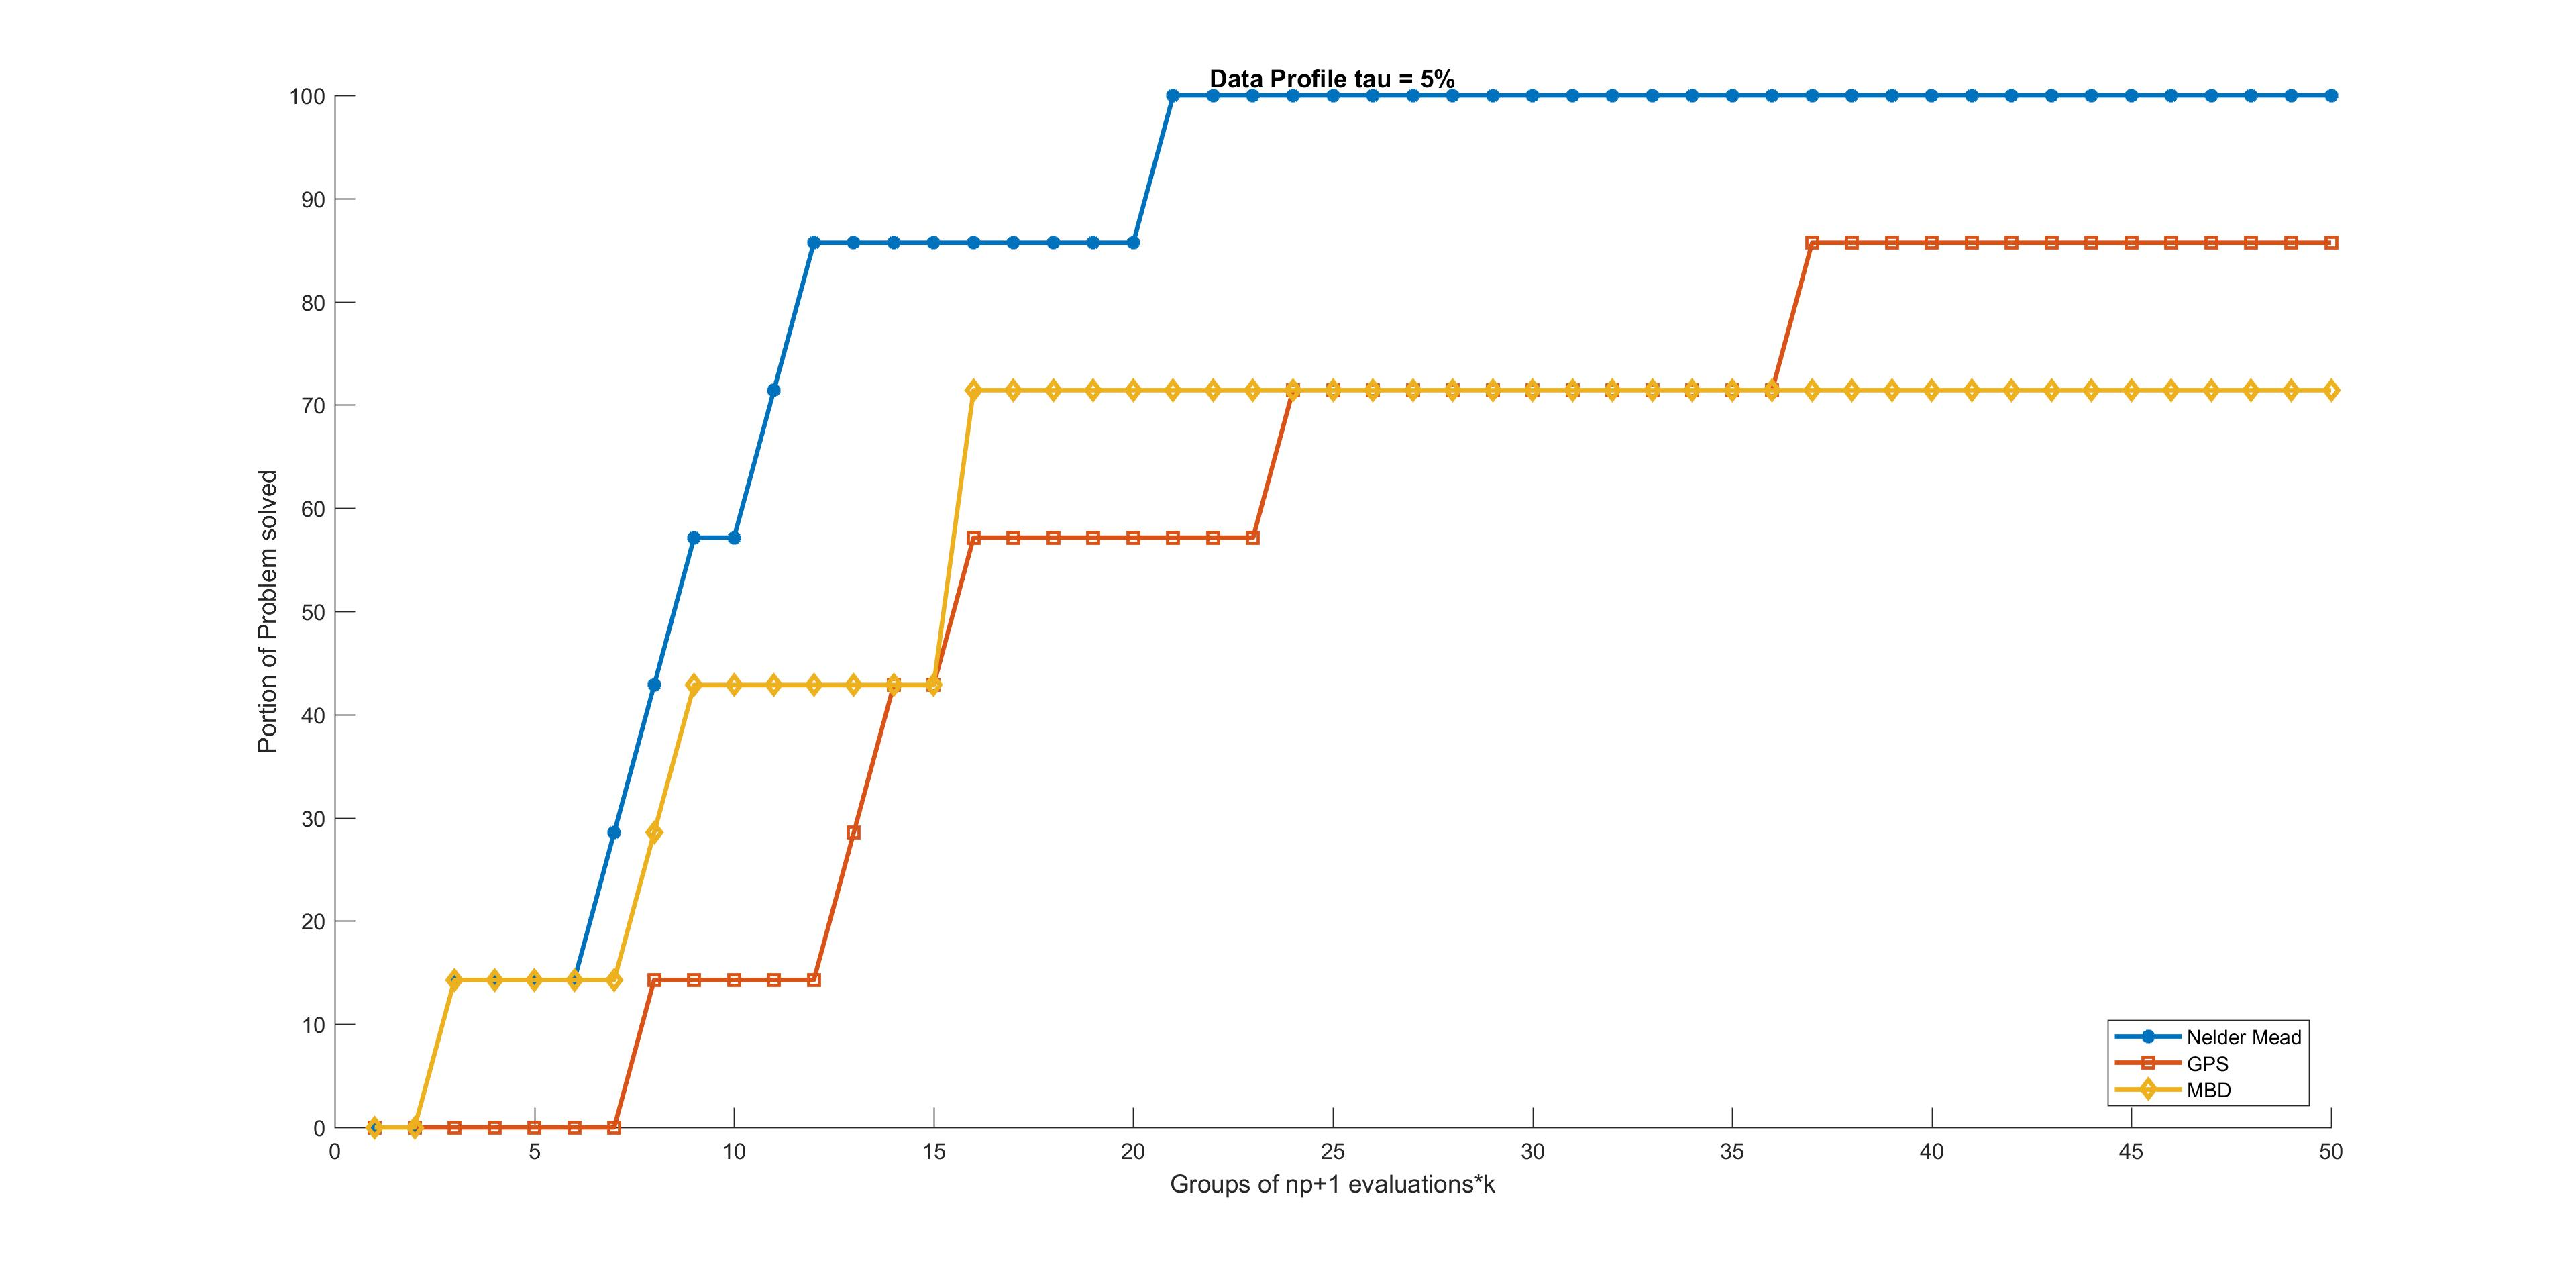
\includegraphics[width=\linewidth]{dptau5.jpg}
			\caption{Data Profile for NM, GPS \& MBD}
		\end{figure}
	\end{frame}

	\begin{frame}{Data Profile}{tau=10\%}
		\begin{figure}
			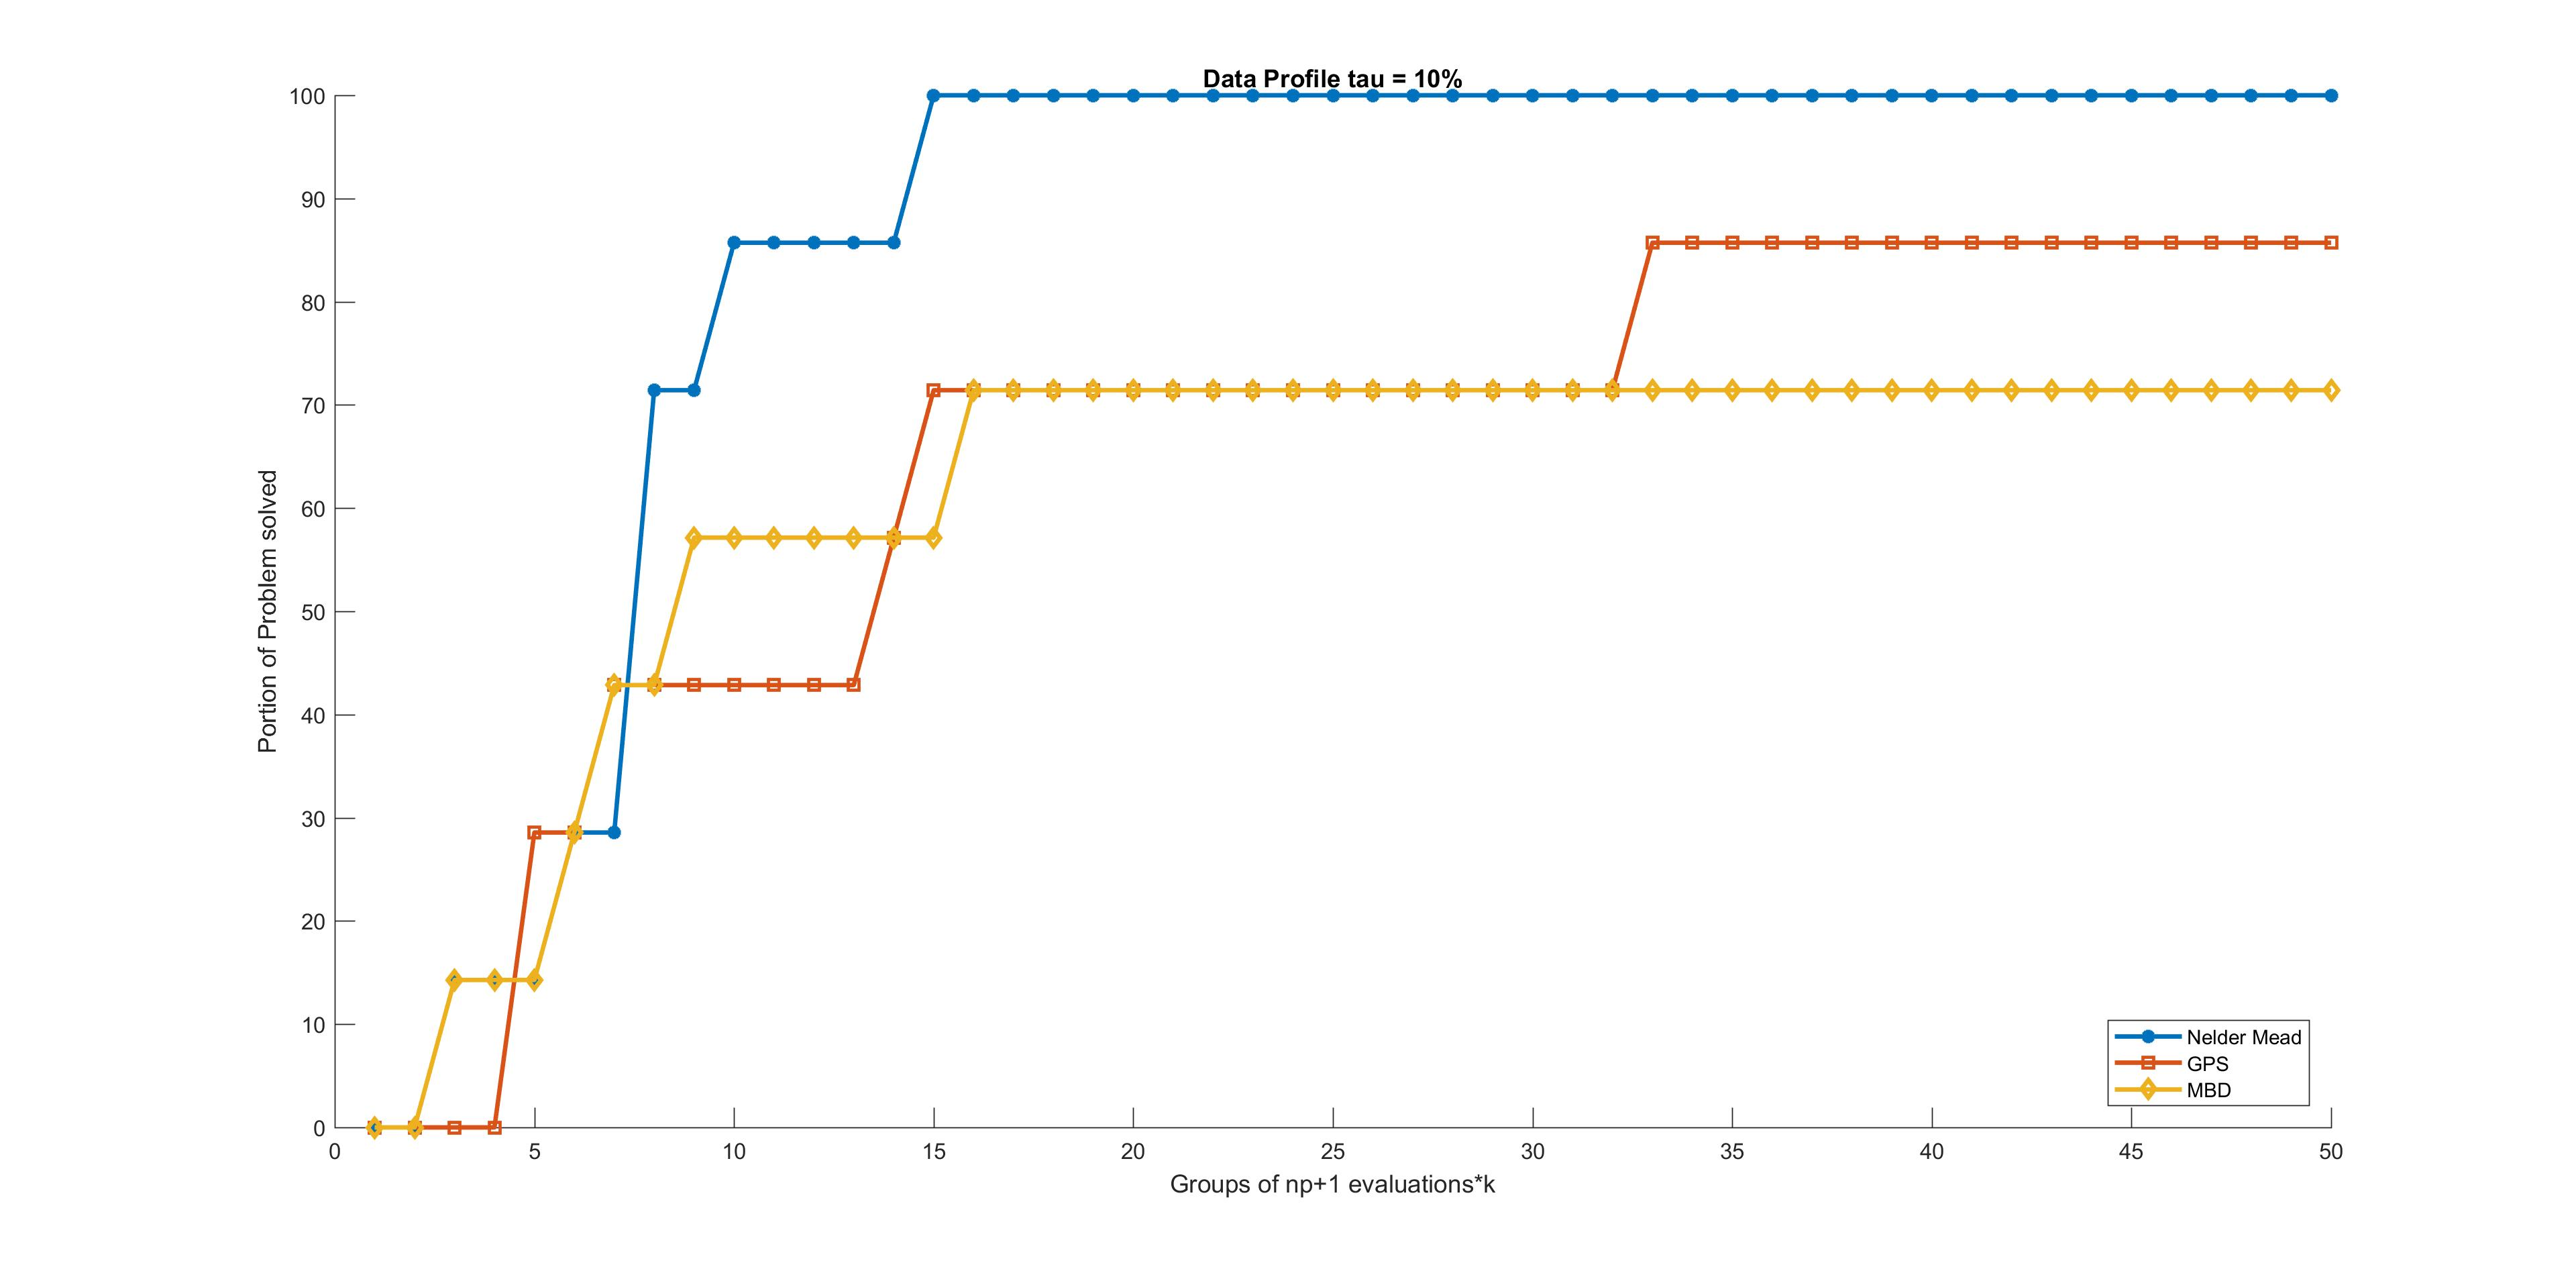
\includegraphics[width=\linewidth]{dptau10.jpg}
			\caption{Data Profile for NM, GPS \& MBD}
		\end{figure}
	\end{frame}

	\begin{frame}{Conclusions}
		In MBD, change in Armijo parameter have a significant impact on the performance of algorithm. A higher value usually makes the algorithm move faster. \\
		When Implemented with standard parameters, Nelder Mead could outperform other Mesh and Model Based Methods.\\
		The set of polling directions matter a lot for GPS. When implemented with $D_{min}$ basis set, it could take as much as twice the functions calls to converge compared to $D_{max} $ set.
		For each iteration, MBD makes lots of function calls because of line search. \\
		MBD (with Linear Regression) is usually quick to reach in $\epsilon$ neighbourhood of the optimum solution (as it uses gradients) but takes a lot of iterations (also dependent on the function) to converge. This is because of inaccuracy of Linear Regression in the computation of approximate gradient. \\
	\end{frame}
	
	\begin{frame}
		\begin{center}
			\begin{Huge}
				Thank You...
			\end{Huge}
		\end{center}
	\end{frame}

\end{document}